\chapter{Results}	\label{ch:results}
\glsresetall
The following sections will present the results obtained using the previously exposed solver in a variety of benchmark cases.
The chosen test cases will be presented incrementally in complexity. In section \cref{ssec:CouetteFlowTempDiff} a Couette flow presenting a temperature gradient in the vertical direction is studied. 
(Subsequently in section XX the temporal discretization is studied using the traditional Taylor-Green vortex.)
In \cref{ss:DHC} a heated square cavity configuration is studied in order to asses the capability of the solver for variable density flows in closed systems. Later in in \cref{ss:CDF} and \cref{ss:CoFlowFlame} two different configurations for reactive flows are presented. 

All calculations shown here where performed on AMD EPYC 7543 32-Core Processor, DDR4 %TODO \todo[inline]{which specifications of the cluster should i include?}





\section{Single-component isothermal cases}
\subsection{ Transpirating Channel?}	
\blindtext[5]
\subsection{ Taylor-Green vortex}
\blindtext[5]



\subsection{Backward-facing step}\label{ssec:BackwardFacingStep}
The backward-facing step problem is a clasical configuration widely used for validation of CFD codes.%and reference data is available in  \cite{armalyExperimentalTheoreticalInvestigation1983} and \cite{xieFluidFlowHeat2016}.
In this section we shall present the results that intend to reproduce the conclusions of the numerical experiments presented in \cite{biswasBackwardFacingStepFlows2004}.

In \cref{BFSsketch} a schematic representation of the problem is shown. 

Although The backward-facing step problem is known to be inherently three-dimensional, it has been shown that it can be studied as a two-dimensional configuration along the symmetry plane for moderate Reynolds numbers \citep{barkleyThreedimensionalInstabilityFlow2000, biswasBackwardFacingStepFlows2004}. For the range of Reynolds numbers used in our calculations the two-dimensional assumption is justified.  The origin of the coordinate system is set at the bottom part of the step. The step height \gls{StepHeigth} and channel height \gls{ChannelHeight} characterize the system. The results on the literature are often reported as a function of the expansion ratio, defined as $\gls{ExpansionRatio} = (\gls{ChannelHeight}+\gls{StepHeigth})/\gls{ChannelHeight}$. 
%For all calculations shown here we set $L = 70 \gls{StepHeigth}$ and $L_0 = \gls{StepHeigth}$.
We conduct a series of simulations with the objective of reproducing the results reported in \cite{biswasBackwardFacingStepFlows2004}, where the backward-facing step was calculated for Reynolds numbers up to $400$ and for a expansion ratio of $1.9423$. 
The Reynolds number for the backward-facing step configuration is defined in the literature in many forms. We adopt here the definition based on the step height \gls{StepHeigth} and mean inlet velocity $U_{\text{mean}}$ as reference values, resulting in
\begin{equation}
\gls{Reynolds}= \frac{\gls{StepHeigth}U_{\text{mean}}}{\gls{kinVisc}}
\end{equation} 
The system is isothermic and the fluid is assumed to be air. The inlet profile is parabolic and is given by
\begin{equation}
u(y) = -6U_{\text{mean}}\frac{(y-S)(y-(h+S))}{h^2}
\end{equation}
%The boundary conditions ??
In order to minimize the effects of the outlet  boundary condition in the system, the length $L$ of the domain was set to $L = 70 \gls{StepHeigth}$. Additionally  $L_0 = \gls{StepHeigth}$. For all calculations in this section an structured grid with 88400 elements is used. To better resolve the complex structures that occur in this configuration, smaller elements are used in the vicinity of the step, as seen in figure \cref{bfsmesh}.

%Preliminary calculations showed that the calculated reattachment and detachment lengths are highly sensitivy to an adequate mesh.
\begin{figure}[tb]
	\begin{center}
		\def\svgwidth{0.9\textwidth}
		\import{./plots/}{BFS_sketch.pdf_tex}		
		\caption{Schematic representation of the backward-facing step. Both primary and secondary vortices are shown. Sketch is not to scale.}
		\label{BFSsketch}
	\end{center}	
\end{figure} 

\begin{figure}[tb]
	\begin{center}
		\def\svgwidth{0.8\textwidth}
		\import{./plots/}{HBFS_MESH.pdf_tex}
		\caption{Structured mesh used in all calculations. }
		\label{bfsmesh}
	\end{center}	
\end{figure} 




\begin{figure}[tb]
	\pgfplotsset{
		group/xticklabels at=edge bottom,
		legend style = {
			at ={ (0.0,0.9), anchor= north west}
		},
		unit code/.code={\si{#1}}
	}
	\centering
	\begin{tikzpicture}
	\begin{groupplot}[
	group style={
		group name=my plots,
		group size=3 by 1,
		x descriptions at=edge bottom,
		ylabels at = edge left,
	},
	width= 0.4\textwidth ,
	height= 0.3\textwidth ,
	xlabel = \gls{Reynolds},
	ylabel= x/S, 
	]
	\nextgroupplot%[title = {\textbf{Primary recirculation zone}}]
	\addplot+[color=black, no marks, thick] table {data/HeatedBackwardFacingStep/BottomReatLength.txt}; \addlegendentry{$R_1$,BoSSS}
	\addplot+[color=black, only marks, dashed]table {data/HeatedBackwardFacingStep/REF_BottomReatLength.txt}; \addlegendentry{$R_1$,Ref}
	\nextgroupplot%[title = {\textbf{Secondary recirculation zone}}]
	\addplot+[color=black, no marks, thick, solid] table {data/HeatedBackwardFacingStep/TopSepLength.txt};  \addlegendentry{$R_2$}
	\addplot+[color=black, no marks, thick, solid] table {data/HeatedBackwardFacingStep/TopReatLength.txt}; \addlegendentry{$R_3$}
	\addplot+[color=black, only marks, dashed]table {data/HeatedBackwardFacingStep/REF_TopSepLength.txt}; \addlegendentry{$R_2$}
	\addplot+[color=black, only marks, dashed]table {data/HeatedBackwardFacingStep/REF_TopReatLength.txt}; \addlegendentry{$R_3$}
	\end{groupplot}
	\end{tikzpicture}
	\caption{ Detachment and reattachment lengths of the primary (left figure) and secondary (right figure) recirculation zones after the backward-facing step. Solid lines correspond to the results obtained with BoSSS and the marks to the reference solution \citep{biswasBackwardFacingStepFlows2004}.}
	\label{fig:Re_De_Attachmentlengths}
\end{figure}
The backward-facing step configuration exhibits varying behaviour as the number of Reynolds changes. At small Reynolds number, a single vortex, usually called the primary vortex, appears in the vicinity of the step. In addition, as the Reynolds number increases, a second vortex eventually appears on the top wall, as is shown schematically in Figure \cref{BFSsketch}. 
The deattachment and reattachment lengths of the vortices are values usually reported in the literature. It is possible to determine the position of deattachment by finding the point along the wall where the velocity gradient u acquires a value equal to zero. %TODO \todo[inline]{comment on this}
Figure \cref{fig:Re_De_Attachmentlengths} shows the deattachment and reattachment lenghts of the primary and secondary vortices obtained with our code for different Reynolds numbers, which are also compared with the results presented in the reference \cite{biswasBackwardFacingStepFlows2004}. It can be observed how the results for the deattachment lengths of the primary vortex present very good agreement with those of the reference. In the case of the secondary vortex it is possible to see a very minimal deviation for the reattachment lenghts. It is interesting to note that despite the fact that the reference does not report the existence of a secondary vortex for $\gls{Reynolds} = 200$, with our code it was possible to observe it. The results allow us to conclude that it is possible to study flows with complex behavior for high Reynolds numbers, at least in the isothermal case. In the next section we will discuss what happens for the non-isothermal case.







\section{Single-component non-isothermal cases}

\subsection{Heated backward-facing step}
As an extension to the previous case, we seek to recreate the results presented in \cite{xieFluidFlowHeat2016}, where the same backward-facing step configuration as presented above is studied, but with the particularity that in this case the bottom wall is heated to a constant temperature, thus featuring a non-isothermal system. The fluid entering the system has a temperature equal to $T_0 = 10°C$ and the bottom wall is set to a constant temperature of $T_1 = 40°C$. 
In \cite{xieFluidFlowHeat2016} results are reported for the local Nusselt numbers and local friction coefficients $f_d$  along the bottom wall for different expansion ratios and Reynolds numbers. The local Nusselt number is defined as
\begin{equation}
\gls{Nusselt} = \frac{S}{T_0-T_1}\nabla T \cdot \vec{n}
\end{equation}
On the other hand, and by recognizing that the wall shear stress along the bottom wall $\tau_{\text{w}} = -\mu \nabla u \cdot \vec{n}$, the local friction factor can be written as
\begin{equation}
f_d = \frac{8\nu} { (U_{\text{mean}})^2}  \nabla u \cdot \vec{n} 
\end{equation}
A series of simulations for varying Reynolds numbers and expansion ratios were conducted. In \cref{BFS_Streamlines} the temperature field and streamlines corresponding to a calculation with $\gls{Reynolds} = 700$ is shown. Here the apparition of the secondary vortex is appreciated. We point out here that the results obtained by us are substantially different from those reported in \cite{xieFluidFlowHeat2016}, and will not be shown here.
Nevertheless, in the work of \cite{henninkLowMachNumberFlow2022} the same is also pointed out, saying that with his method it was not possible to reproduce the results presented by \cite{xieFluidFlowHeat2016}. Comparing our results with those of Hennink we can see that the same results are obtained, as demonstrated in \cref{fig:fd_Nu_plot}.

\begin{figure}[tb]
	\begin{center}
		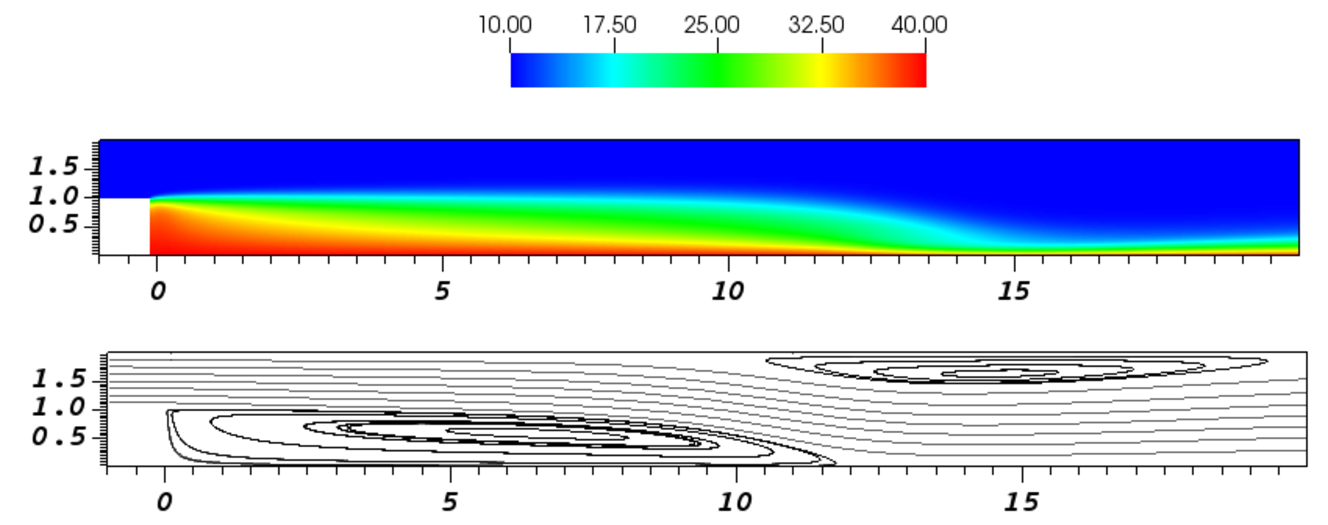
\includegraphics[width=\linewidth]{../plots/HBFS_TemperatureRe700.pdf}
		\caption{Temperature profile (top) and streamlines (bottom) corresponding to the backward-facing Step configuration for $\gls{Reynolds} = 400$ and an expansion ratio of two.}
		\label{BFS_Streamlines}
	\end{center}	
\end{figure} 

\begin{figure}[tb]
	\pgfplotsset{
		group/xticklabels at=edge bottom,
		legend style = {
			at ={ (0.59,1.0), anchor= north east}
		},
		unit code/.code={\si{#1}}
	}
	\begin{tikzpicture}
	\begin{axis}[
	width= 0.4\textwidth ,
	height= 0.3\textwidth ,
	xlabel = x,
	ylabel= $f_d$, 
	]
	\addplot+[color=black, no marks, thick] table {data/HeatedBackwardFacingStep/fd700.txt}; \addlegendentry{BoSSS}
	\addplot+[color=black, only marks, dashed]table {data/HeatedBackwardFacingStep/REF_fd700.txt}; \addlegendentry{Reference}
	\end{axis}
	\end{tikzpicture}
	\begin{tikzpicture}
	\begin{axis}[
	width= 0.4\textwidth ,
	height= 0.3\textwidth ,
	xlabel = x,
	ylabel= \gls{Nusselt}, 
	]
	\addplot+[color=black, no marks, thick] table {data/HeatedBackwardFacingStep/Nu700.txt}; \addlegendentry{BoSSS}
	\addplot+[color=black, only marks, dashed]table {data/HeatedBackwardFacingStep/REF_Nu700.txt}; \addlegendentry{Reference}
	\end{axis}
	\end{tikzpicture}
	\caption{ Local friction factor and local Nusselt number along the bottom wall for $\gls{Reynolds} = 700$ and an expansion ratio of two. The solid lines corresponds to our solution and the marks to the reference \cite{henninkLowMachNumberFlow2022}}
	\label{fig:fd_Nu_plot}
\end{figure}

\begin{figure}[tb]
\centering
	\pgfplotsset{
		group/xticklabels at=edge bottom,
		legend style = {
			at ={ (0.59,1.0), anchor= north east}
		},
		unit code/.code={\si{#1}}
	}
	\begin{tikzpicture}
	\begin{axis}[
	width= 0.4\textwidth ,
	height= 0.3\textwidth ,
	xlabel = x,
	ylabel= $f_d$, 
	]
	\addplot+[color=black, no marks, thick] table {data/HeatedBackwardFacingStep/VelXArr7.txt};
	\addplot+[color=black, no marks, thick] table {data/HeatedBackwardFacingStep/VelXArr15.txt};
	\addplot+[color=black, only marks, thick] table {data/HeatedBackwardFacingStep/VelXArr7_REF.txt}; 
	\addplot+[color=black, only marks, thick] table {data/HeatedBackwardFacingStep/VelXArr15_REF.txt};	
	%	 \addlegendentry{Reference}y
	\end{axis}
	\end{tikzpicture}
	\caption{bla}
	\label{fig:uvelBFS}
\end{figure}

\FloatBarrier

\subsection{Couette flow with vertical temperature gradient} \label{ssec:CouetteFlowTempDiff}
\begin{figure}[tb]
	\begin{center}
		\def\svgwidth{0.5\textwidth}
		\import{./plots}{HeatedCouetteSketch.pdf_tex}
		\caption{Schematic representation of the couette flow with temperature difference test case.}
		\label{fig:CouetteTempDiff_scheme}
	\end{center}	
\end{figure} 

As a first benchmark case to test the implemented low-Mach solver we analyse the Couette flow with a vertical temperature gradient. This configuration was already studied in \citep{kleinHighorderDiscontinuousGalerkin2016}, where the SIMPLE algorithm in a DG framework was used. We intend in this section to reproduce their results by using our fully coupled solver. 
We also show later how our implemented solver performs in relation to the SIMPLE based solver.% by comparing runtimes 

In \cref{fig:CouetteTempDiff_scheme} a schematic representation of the testcase is shown. The top wall corresponds to a moving wall ($u = 1$) with a fixed temperature $T=T_h$. The bottom wall is a static one ($u = 0$), and has a constant temperature $T = T_c$. 
The domain is chosen as $\Omega = [0,1]\times[0,1]$, and Dirichlet boundary conditions are used for all boundaries. It is assumed that the fluid is composed of only one component, thus $\gls{TotalNumberSpecies} = 1$ and we can prescribe $Y_0 = 1.0$ everywhere in the domain. Additionally,the system is subjected to a gravitational field, where the gravity vector only has a component in the $y$ direction. Under this conditions, the x-velocity, pressure and temperature are only dependent on the $y$ coordinate, i.e. $u = u(y)$, $T = T(y)$ and $p = p(y)$. Thus, the governing equations (\cref{eq:NS-eq}) reduce to 
\begin{align}
&\frac{1}{\gls{Reynolds}} \pfrac{ }{y}\left(\mu\pfrac{u}{y}\right) = 0,\\
&\pfrac{p}{y} = -\frac{\gls{dens}}{\gls{Froude}^2},\\
&\frac{1}{\gls{Reynolds}~\gls{Prandtl}} \pfrac{ }{y}\left(\gls{HeatConductivity}\pfrac{T}{y}\right) = 0.
\end{align}
It is possible to find an analytical solution for this problem.
%%Constant transport properties
%By assuming $\gls{Prandtl} = 1.0$ and constant transport properties ($\mu = \lambda = 1$), we can derive the analytical solution of XXX
%\begin{align}
%u &= y,\\
%p &= - \frac{p0}{\gls{Froude}^2(T_h-T_c)}\ln\left((T_h-T_c)y+T_c\right)+C,\\
%T &= (T_h-T_c)y + T_c,
%\end{align}
%where $C$ is an arbitrary constant which defines the mean value of the pressure TODO rewritethis.
% Variable transport properties
By assuming a temperature dependence of the transport properties according a Power Law ($\mu = \lambda = T^{2/3}$) a solution is obtained as 
\begin{align}
u(y) &= C_1 + C_2\left(y + \frac{T_c^{5/3}}{T_h^{5/3}-T_c^{5/3}} \right)^{3/5},\label{eq:CouetteU}\\
p(y) &= -\frac{5p_0}{2\gls{Froude}^2}\frac{\left(y\left(T_h^{5/3}-T_c^{5/3}\right)+T_c^{5/3}\right)^{2/5}}{\left(T_h^{5/3}-T_c^{5/3}\right)}+C,\label{eq:Couettep}\\
T(y) &= \left(C_3 - \frac{5}{3}C_4 y\right)^{3/5}\label{eq:CouetteT}.
\end{align} 
Where the constants $C_1$, $C_2$, $C_3$ and $C_4$ are determined by using the boundary conditions on the top and bottom walls, and are given by 
\begin{align}
C_1 &= \frac{\left(\frac{T_c^{5/3}}{T_h^{5/3}-T_c^{5/3}}\right)^{3/5}}{\left(\frac{T_c^{5/3}}{T_h^{5/3}-T_c^{5/3}}\right)^{3/5}-\left(\frac{T_h^{5/3}}{T_h^{5/3}-T_c^{5/3}}\right)^{3/5}}\\
C_2 &= \frac{1}{\left(\frac{T_h^{5/3}}{T_h^{5/3}-T_c^{5/3}}\right)^{3/5}-\left(\frac{T_c^{5/3}}{T_h^{5/3}-T_c^{5/3}}\right)^{3/5}}\\
C_3 &= T_c^{5/3},\\
C_4 &= \frac{3}{5}\left(T_c^{5/3}-T_h^{5/3}\right)
\end{align}
and again $C$ is a real-valued arbitrary constant for the pressure. 
\begin{center}
	\begin{table}[tb!]
		\begin{tabular}{ccc}
			\begin{tikzpicture}[baseline]
			\begin{axis}[
			xmin = 0, xmax = 1, ymin =0, ymax=1,
			width= 0.2\textwidth ,
			height= 0.22\textwidth ,
			xlabel = y,
			ylabel= u, 
			]
			\addplot+[color=black, no marks, thick] table {data/CouetteTempDifferenceData/u.txt};
			\end{axis}
			\end{tikzpicture}%
			&
			\begin{tikzpicture}[baseline]
			\begin{axis}[
			xmin = 0, xmax = 1, %ymin =0, ymax=1,
			width= 0.2\textwidth ,
			height= 0.22\textwidth ,
			xlabel = y,
			ylabel= p, 
			]
			\addplot+[color=black, no marks, thick] table {data/CouetteTempDifferenceData/p.txt};
			\end{axis}
			\end{tikzpicture}%
			&
			\begin{tikzpicture}[baseline]
			\begin{axis}[
			xmin = 0, xmax = 1, ymin =0.4, ymax=1.6,
			width= 0.2\textwidth ,
			height= 0.22\textwidth ,
			xlabel = y,
			ylabel= T, 
			]
			\addplot+[color=black, no marks, thick] table {data/CouetteTempDifferenceData/T.txt};
			\end{axis}
			\end{tikzpicture}%
		\end{tabular}%
		\caption{Solution of the Couette flow with vertical temperature gradient. Viscosity and heat conductivity are calculated with a Power-Law.}
		\label{fig:CouetteSolution}
	\end{table}
\end{center}
\FloatBarrier
For all calculations of this configuration shown in the following sections the dimensionless parameters are set as $\gls{Reynolds} = 10$ and $\gls{Prandtl} =0.71$, $T_h = 1.6$ and $T_c = 0.4$. Since we are dealing with an open system we set $p_0 =1.0$. The Froude number is calculated as 
\begin{equation}
\text{Fr} = \left( \frac{2\text{Pr}(T_h-T_c)}{(T_h+T_c)}\right)^{1/2}
\end{equation}
In \cref{fig:CouetteSolution} the solution for the velocity, pressure and temperature are shown. The results are for a mesh with $26\times26$ elements and a polynomial degree of three for $u$ and $T$, and a polynomial degree of two for $p$.
%\pgfplotsset{
%	small,
%}


\subsubsection{h-convergence study}

The convergence properties of the DG method for this non-isothermic system was studied using the analytical solution described before. The domain is discretized and solved in uniform Cartesian meshes with $16\times16$, $32\times32$, $64\times64$ and $128\times128$ elements. The polynomial degrees for the velocity and temperature are changed from 1 to 4 and for the pressure from 0 to 3. The convergence criteria described in \cref{ssec:TerminationCriterion} was used for all calculations. The  analytical solution given by \cref{eq:CouetteU,eq:Couettep,eq:CouetteT} are as Dirichlet boundary conditions on all boundaries of the domain. The error is calculated against the analytical solution using the $L^2$ norm %TODO \todo[inline]{Comment more on the calculation of the l2norm}.
In \cref{fig:ConvergenceDHC} the results of the h-convergence study are shown. We observe how the expected convergence rates are reached for all variables, namely a slope of the order $k+1$ for both velocity components and the temperature, and a slope of $k'+1$ for the pressure.

%

\subsubsection{Convergence study}\label{ssec:ConvStudyHeatedCavity}
An $h-$convergence study of the XNSEC solver was conducted using the heated cavity configuration. Calculations were performed for polynomial degrees $k = {1,2,3,4}$ and equidistant regular meshes with, respectively, $8\times8$, $16\times16$, $32\times32$, $64\times64$, $128\times128$ and $256\times256$ elements.  The $L^2$ -Norm was used to calculate errors against the solution in the finest mesh. The results of the $h$-convergence study for varying polynomial orders $k$ are shown in \cref{fig:ConvergenceDHC}. It is observed how the convergence rates scale approximately as $k+1$. Interestingly, for $k=2$ the rates are higher than expected. On the other hand, some degeneration is observed in convergence rates for $k = 4$. This strange behavior can be explained if one considers that the heated cavity presents a singular behavior at the corners (similar to the problem previously exposed for the lid-driven cavity), which causes global pollution in the convergence behavior of the algorithm. 
 
As discussed in the previous section, the difference in the average values of the Nusselt number on the hot wall $\text{Nu}_\text{h}$  and the cold wall $\text{Nu}_\text{c}$ is a direct consequence of the spatial discretization error and should decrease for finer meshes. In \cref{fig:NusseltStudy} the convergence behavior of the Nusselt number is presented for different polynomial degrees $k$, different number of elements and for two Rayleigh numbers. As expected, it can be observed that this discrepancy is smaller when a larger number of elements is used. It can also be seen that  $\text{Nu}_\text{h}$ reaches the expected solution of cells for a much smaller number of elements. This can be explained if one thinks that more complex phenomena take place near the cold wall (see \cref{fig:HSCStreamlines}), which makes necessary a finer mesh resolution in that area.



\begin{figure}[tb]
	\centering
	\pgfplotsset{width=0.34\textwidth, compat=1.3}
	\inputtikz{ConvergenceDHC}
	\caption{Convergence study of the differentially heated cavity problem for $\text{Ra} = 10^3$.}\label{fig:ConvergenceDHC}
\end{figure}
\begin{figure}[tb]
	\centering
	\inputtikz{NusseltStudy}
	\caption[Nusselt numbers of the differentially heated square cavity at the hot wall ($\text{Nu}_h$) and the cold wall ($\text{Nu}_c$) for different number of cells and polynomial order $k$.]{Nusselt numbers of the differentially heated square cavity at the hot wall ($\text{Nu}_h$) and the cold wall ($\text{Nu}_c$) for different number of cells and polynomial order $k$. The reference values from \textcite{vierendeelsBenchmarkSolutionsNatural2003} are shown with dashed lines.}\label{fig:NusseltStudy}
\end{figure}
\FloatBarrier
\subsubsection{Influence of the penalty factor}
\begin{table}[h]
\centering
\begin{tabular}{lllllll}
	\hline \vspace{0.1cm}
		$\eta_0$                  &  $k$ & DOFs& $\text{Nu}_c$ &  $\frac{\text{Nu}_c - \text{Nu}_{c,\text{ref}}} {\text{Nu}_{c,\text{ref}}}\times 10^2 $   & $p_0$    & $\frac{p_0 - p_{0,\textbf{ref}}} {p_{0,\textbf{ref} }}\times 10^4 $ \\ \hline
\multirow{3}{*}{0.01} & 2 & 6804 & 0.549483* & 50.39424 & 0.899757* & 408.7292 \\
                      & 3 & 7056 & 0.722593* & 34.76637 & 0.936085* & 21.48436 \\
                      & 4 & 6655 & -0.50954* & 146      & 1.016691* & 837.7683 \\ \hline
\multirow{3}{*}{1}    & 2 & 6804 & 1.090047 & 1.593667 & 0.938192 & 0.980674 \\
                      & 3 & 7056 & 1.102072 & 0.508037 & 0.938057 & 0.453674 \\
                      & 4 & 6655 & 1.105225 & 0.22348  & 0.938046 & 0.570494 \\ \hline
\multirow{3}{*}{4}    & 2 & 6804 & 1.089332 & 1.65817  & 0.93843  & 3.521926 \\
                      & 3 & 7056 & 1.102261 & 0.491027 & 0.938076 & 0.25384  \\
                      & 4 & 6655 & 1.105359 & 0.211372 & 0.938047 & 0.561709 \\ \hline
\multirow{3}{*}{16}   & 2 & 6804 & 1.08694  & 1.874166 & 0.939109 & 10.75641 \\
                      & 3 & 7056 & 1.102266 & 0.490563 & 0.938124 & 0.251627 \\
                      & 4 & 6655 & 1.105439 & 0.204153 & 0.93805  & 0.537265 \\ \hline
\end{tabular}
\caption[Thermodynamic pressure and cold-side Nusselt number for different penalty safety factors in a heated cavity with Ra $=10^3$.]{Thermodynamic pressure and cold-side Nusselt number for different penalty safety factors in a heated cavity with Ra $=10^3$. Values marked with an asterisk are from problems not converged after 100 iterations.} \label{fig:EtaInfluence}
\end{table}
A point not still discussed is the choice of the safety parameter $\eta_0$ of the penalty terms from the SIP discretization (see \cref{eq:PenaltyFactor}).  \Cref{fig:EtaInfluence} shows results obtained for Ra $=10^3$, for different polynomial degrees and penalty safety factor.  For the tests presented here, the penalty terms of the diffusive terms from the momentum and energy equations are considered equal. Furthermore, the number of elements in the mesh is selected in such a way that the number of degrees of freedom remains approximately constant for each simulation. 

It is possible to see that the penalty safety factor (and therefore the penalty term) can have a great influence on the solution. If the value chosen is very small, as in the case of the table for $\eta_0 = 0.01$, the algorithm is not able to find a solution. On the other hand, if the chosen value is too high, the error also increases. It can be concluded that an optimal value for the penalty factor exists.

It is also noticeable that, maintaining a constant penalty safety factor, increasing the polynomial degree for an approximately constant number of DOFs gives an improvement in the results compared to the literature. Although for this testcase the effect of the penalty factor on the solution is not very large, the effect could be considerable, especially when dealing with more complex geometries and coarser meshes. The value $\eta_0 = 4$ has shown to be a value that gives stability to the scheme and is used for all simulations in this thesis, as already has been done in many works \parencite{krauseIncompressibleImmersedBoundary2017,kummerExtendedDiscontinuousGalerkin2017,smudamartinDirectNumericalSimulation2021} and is used for all calculations in this work.
 
The results presented in this section allows to conclude that the implemented solver is capable of dealing with flows with variable densities, and in particular in closed spaces. Additionally, it was observed that even for this complex test, convergence properties close to those expected from the DG method are obtained. Until this point only systems with a steady state solution were treated. Later in \cref{ssec:FlowCircCyl} the ability of the solver to compute flows with varying densities in non-steady state will be shown.


\begin{figure}[t!]
	\centering
	\pgfplotsset{width=0.34\textwidth, compat=1.3}
	\begin{tikzpicture}
		\begin{groupplot}[
			group style={
				group name= group,
				group size=2 by 2,
				ylabels at=edge left,
				horizontal sep = 2.5cm,
				vertical sep = 1.5cm,
			},
			xtick={2^-8,2^-7,2^-6, 2^-5, 2^-4,2^-3},
			xticklabels = {$2^{-8}$,$2^{-7}$,$2^{-6}$,$2^{-5}$, $2^{-4}$, $2^{-3}$},
			xlabel=Cell length $h$,
			xmajorgrids,
			ymajorgrids,
			legend style={at={(1,0)}, anchor=south east},
			]
			\nextgroupplot[xmode=log, ymode=log,ylabel = $\LtwoNorm{ u_x - u_{x,\text{fine}}}$,]
			\addplot+[color=black, dashed] table {data/ConvStudy_Couette_PowerLaw/VelocityXDG1Data.txt};
			\addlegendentry{$k=1$};
			\addplot[solid,  forget plot] table [   
			x=x,
			y={create col/linear regression={y=y,
					variance list={10000,800,600,500,400,200,100}}}]
			{data/ConvStudy_Couette_PowerLaw/VelocityXDG1Data.txt}
			coordinate [pos=0.75] (A)
			coordinate [pos=0.90] (B)
			;
			\xdef\slopeXA{\pgfplotstableregressiona}			
			\draw (A) |- (B)
			node [pos=0.55,anchor= west]
			{\pgfmathprintnumber{\slopeXA}};			
			\addplot+[color=black, dashed] table {data/ConvStudy_Couette_PowerLaw/VelocityXDG2Data.txt};
			\addlegendentry{$k=2$};
			\addplot[solid, forget plot] table [   
			x=x,
			y={create col/linear regression={y=y,
					variance list={10000,800,600,500,400,200,100}				
			}}]
			{data/ConvStudy_Couette_PowerLaw/VelocityXDG2Data.txt}
			coordinate [pos=0.75] (A)
			coordinate [pos=0.90] (B)
			;
			\xdef\slopeXB{\pgfplotstableregressiona}			
			\draw (A) |- (B)
			node [pos=0.15,anchor=  west]
			{\pgfmathprintnumber{\slopeXB}};			
			\addplot+[color=black, dashed] table {data/ConvStudy_Couette_PowerLaw/VelocityXDG3Data.txt};
			\addlegendentry{$k=3$};			
			\addplot[solid, forget plot] table [   
			x=x,
			y={create col/linear regression={y=y,
					variance list={10000,800,600,500,400,200,100}}}]
			{data/ConvStudy_Couette_PowerLaw/VelocityXDG3Data.txt}
			coordinate [pos=0.80] (A)
			coordinate [pos=0.95] (B)
			;
			\xdef\slopeXC{\pgfplotstableregressiona}			
			\draw (A) |- (B)
			node [pos=0,anchor=east]
			{\pgfmathprintnumber{\slopeXC}};			
			\addplot+[color=black, dashed] table {data/ConvStudy_Couette_PowerLaw/VelocityXDG4Data.txt};
			\addlegendentry{$k=4$};
			\addplot[solid, forget plot] table [   
			x=x,
			y={create col/linear regression={y=y,
					variance list={10000,800,600,500,400,200,100}}}]
			{data/ConvStudy_Couette_PowerLaw/VelocityXDG4Data.txt}
			coordinate [pos=0.75] (A)
			coordinate [pos=0.9] (B)
			;
			\xdef\slopeXD{\pgfplotstableregressiona}			
			\draw (A) |- (B)
			node [pos=0.55,anchor=south west]
			{\pgfmathprintnumber{\slopeXD}};	
			\nextgroupplot[xmode=log, ymode=log,	ylabel = $\LtwoNorm{ u_y - u_{y,\text{fine}}}$,]
			\addplot+[color=black, dashed] table {data/ConvStudy_Couette_PowerLaw/VelocityYDG1Data.txt};
			\addlegendentry{$k=1$};
			\addplot[solid,  forget plot] table [   
			x=x,
			y={create col/linear regression={y=y,
					variance list={10000,800,600,500,400,200,100}}}]
			{data/ConvStudy_Couette_PowerLaw/VelocityYDG1Data.txt}
			coordinate [pos=0.75] (A)
			coordinate [pos=0.90] (B)
			;
			\xdef\slopeXA{\pgfplotstableregressiona}			
			\draw (A) |- (B)
			node [pos=0.55,anchor= west]
			{\pgfmathprintnumber{\slopeXA}};			
			\addplot+[color=black, dashed] table {data/ConvStudy_Couette_PowerLaw/VelocityYDG2Data.txt};
			\addlegendentry{$k=2$};
			\addplot[solid, forget plot] table [   
			x=x,
			y={create col/linear regression={y=y,
					variance list={10000,800,600,500,400,200,100}}}]
			{data/ConvStudy_Couette_PowerLaw/VelocityYDG2Data.txt}
			coordinate [pos=0.75] (A)
			coordinate [pos=0.90] (B)
			;
			\xdef\slopeXB{\pgfplotstableregressiona}			
			\draw (A) |- (B)
			node [pos=0.55,anchor=  west]
			{\pgfmathprintnumber{\slopeXB}};			
			\addplot+[color=black, dashed] table {data/ConvStudy_Couette_PowerLaw/VelocityYDG3Data.txt};
			\addlegendentry{$k=3$};			
			\addplot[solid, forget plot] table [   
			x=x,
			y={create col/linear regression={y=y,
					variance list={10000,800,600,500,400,200,100}}}]
			{data/ConvStudy_Couette_PowerLaw/VelocityYDG3Data.txt}
			coordinate [pos=0.75] (A)
			coordinate [pos=0.90] (B)
			;
			\xdef\slopeXC{\pgfplotstableregressiona}			
			\draw (A) |- (B)
			node [pos=0.55,anchor=south west]
			{\pgfmathprintnumber{\slopeXC}};			
			\addplot+[color=black, dashed] table {data/ConvStudy_Couette_PowerLaw/VelocityYDG4Data.txt};
			\addlegendentry{$k=4$};
			\addplot[solid, forget plot] table [   
			x=x,
			y={create col/linear regression={y=y,
					variance list={10000,800,600,500,400,200,100}}}]
			{data/ConvStudy_Couette_PowerLaw/VelocityYDG4Data.txt}
			coordinate [pos=0.75] (A)
			coordinate [pos=0.9] (B)
			;
			\xdef\slopeXD{\pgfplotstableregressiona}			
			\draw (A) |- (B)
			node [pos=0.55,anchor=south west]
			{\pgfmathprintnumber{\slopeXD}};	
			\nextgroupplot[ xmode=log, ymode=log,	ylabel=$ \LtwoNorm{T - T_{\text{fine}}}$,]
			\addplot+[color=black, dashed] table {data/ConvStudy_Couette_PowerLaw/TemperatureDG1Data.txt};
			\addlegendentry{$k=1$};
			\addplot[solid,  forget plot] table [   
			x=x,
			y={create col/linear regression={y=y,
					variance list={10000,800,600,500,400,200,100}}}]
			{data/ConvStudy_Couette_PowerLaw/TemperatureDG1Data.txt}
			coordinate [pos=0.75] (A)
			coordinate [pos=0.90] (B)
			;
			\xdef\slopeXA{\pgfplotstableregressiona}			
			\draw (A) |- (B)
			node [pos=0.55,anchor= west]
			{\pgfmathprintnumber{\slopeXA}};			
			\addplot+[color=black, dashed] table {data/ConvStudy_Couette_PowerLaw/TemperatureDG2Data.txt};
			\addlegendentry{$k=2$};
			\addplot[solid, forget plot] table [   
			x=x,
			y={create col/linear regression={y=y,
					variance list={10000,800,600,500,400,200,100}}}]
			{data/ConvStudy_Couette_PowerLaw/TemperatureDG2Data.txt}
			coordinate [pos=0.75] (A)
			coordinate [pos=0.85] (B)
			;
			\xdef\slopeXB{\pgfplotstableregressiona}			
			\draw (A) |- (B)
			node [pos=0.55,anchor=  west]
			{\pgfmathprintnumber{\slopeXB}};			
			\addplot+[color=black, dashed] table {data/ConvStudy_Couette_PowerLaw/TemperatureDG3Data.txt};
			\addlegendentry{$k=3$};			
			\addplot[solid, forget plot] table [   
			x=x,
			y={create col/linear regression={y=y,
					variance list={10000,800,600,500,400,200,100}}}]
			{data/ConvStudy_Couette_PowerLaw/TemperatureDG3Data.txt}
			coordinate [pos=0.75] (A)
			coordinate [pos=0.90] (B)
			;
			\xdef\slopeXC{\pgfplotstableregressiona}			
			\draw (A) |- (B)
			node [pos=0.55,anchor=south west]
			{\pgfmathprintnumber{\slopeXC}};			
			\addplot+[color=black, dashed] table {data/ConvStudy_Couette_PowerLaw/TemperatureDG4Data.txt};
			\addlegendentry{$k=4$};
			\addplot[solid, forget plot] table [   
			x=x,
			y={create col/linear regression={y=y,
					variance list={100000,800000,600,500,400,200,100}}}]
			{data/ConvStudy_Couette_PowerLaw/TemperatureDG4Data.txt}
			coordinate [pos=0.75] (A)
			coordinate [pos=0.9] (B)
			;
			\xdef\slopeXD{\pgfplotstableregressiona}			
			\draw (A) |- (B)
			node [pos=0.55,anchor=south west]
			{\pgfmathprintnumber{\slopeXD}};
			\nextgroupplot[xmode=log, ymode=log,ylabel=$\LtwoNorm{ p - p_{\text{fine}} }$,]
			\addplot+[color=black, dashed] table {data/ConvStudy_Couette_PowerLaw/PressureDG1Data.txt};
			\addlegendentry{$k'=0$};
			\addplot[solid,  forget plot] table [   
			x=x,
			y={create col/linear regression={y=y,
					variance list={10000,800,600,500,400,200,100}}}]
			{data/ConvStudy_Couette_PowerLaw/PressureDG1Data.txt}
			coordinate [pos=0.75] (A)
			coordinate [pos=0.90] (B)
			;
			\xdef\slopeXA{\pgfplotstableregressiona}			
			\draw (A) |- (B)
			node [pos=0.55,anchor= west]
			{\pgfmathprintnumber{\slopeXA}};			
			\addplot+[color=black, dashed] table {data/ConvStudy_Couette_PowerLaw/PressureDG2Data.txt};
			\addlegendentry{$k'=1$};
			\addplot[solid, forget plot] table [   
			x=x,
			y={create col/linear regression={y=y,
					variance list={10000,800,600,500,400,200,100}}}]
			{data/ConvStudy_Couette_PowerLaw/PressureDG2Data.txt}
			coordinate [pos=0.80] (A)
			coordinate [pos=0.95] (B)
			;
			\xdef\slopeXB{\pgfplotstableregressiona}			
			\draw (A) |- (B)
			node [pos=0, anchor =east]
			{\pgfmathprintnumber{\slopeXB}};			
			\addplot+[color=black, dashed] table {data/ConvStudy_Couette_PowerLaw/PressureDG3Data.txt};
			\addlegendentry{$k'=2$};			
			\addplot[solid, forget plot] table [   
			x=x,
			y={create col/linear regression={y=y,
					variance list={10000,800,600,500,400,200,100}}}]
			{data/ConvStudy_Couette_PowerLaw/PressureDG3Data.txt}
			coordinate [pos=0.75] (A)
			coordinate [pos=0.90] (B)
			;
			\xdef\slopeXC{\pgfplotstableregressiona}			
			\draw (A) |- (B)
			node [pos=0.55,anchor=south west]
			{\pgfmathprintnumber{\slopeXC}};			
			\addplot+[color=black, dashed] table {data/ConvStudy_Couette_PowerLaw/PressureDG4Data.txt};
			\addlegendentry{$k'=3$};
			\addplot[solid, forget plot] table [   
			x=x,
			y={create col/linear regression={y=y,
					variance list={10000,800,600,500,400,200,100}}}]
			{data/ConvStudy_Couette_PowerLaw/PressureDG4Data.txt}
			coordinate [pos=0.75] (A)
			coordinate [pos=0.9] (B)
			;
			\xdef\slopeXD{\pgfplotstableregressiona}			
			\draw (A) |- (B)
			node [pos=0.55,anchor=south west]
			{\pgfmathprintnumber{\slopeXD}};		
		\end{groupplot}
	\end{tikzpicture}
	\caption{Convergence study of the differentially heated cavity problem for $\text{Ra} = 10^3$.}\label{fig:ConvergenceDHC}
\end{figure}

\subsubsection{Comparison with SIMPLE}
As mentioned before, a solver for solving low-Mach flows based on the SIMPLE algorithm (presented in \cite{kleinHighorderDiscontinuousGalerkin2016}) has been already developed and implemented within the BoSSS framework. 
Though the solver was validated and shown to be useful for a wide variety of test cases, there were also disadvantages inherently associated with the SIMPLE algorithm. Within the solution algorithm, Picard-type iterations are used to search for a solution. This requires some prior knowledge from the user in order to select suitable relaxation factor values that provide stability to the algorithm, but at the same time do not slow down the computation substantially.
It was also observed that the calculation times were prohibitively high for some test cases. This point motivated the development of the solver presented in the present work, where the system is solved in a monolytic way and  and the Newton method globalized with a Dogleg-type method is used to solve the system.  
%TODO \todo[inline]{what are exactly the advantages of the present solver? multigrid? Ortogonalization?} 
We intend to show in this section a comparison of runtimes of the calculation of the Couette flow with vertical temperature gradient between the DG-SIMPLE algorithm \citep{kleinHighorderDiscontinuousGalerkin2016} and the present solver (denoted here as XNSEC). Calculations were performed on uniform Cartesian meshes with $16\times16$, $32\times32$, $64\times64$ and $128\times128$ elements, and with varying polynomial degrees between 1 and 3 for the velocity and temperature, and between 0 y 2 for the pressure. All calculations where initialized with a zero velocity and pressure field, and with a temperature equal to one in the whole domain. Are calculations were performed single-core and the convergence criteria is set to $10^{-8}$ for both solvers. The under-relaxation factors for the SIMPLE algorithm were set for all calculations to 0.8, 0.5 and 1.0 for the velocity, pressure and temperature, respectively. 

In figure \cref{fig:RuntimeComparison} a comparison of the runtimes from both solvers is shown. It is clearly  appreciated how the runtimes of the SIMPLE algorithm are higher for almost all of the cases studied. Obviously the under-relaxation parameters of the SIMPLE algorithm have an influence on the calculation times and an appropiate selection of them could decrease the runtimes. This is a clear disadvantage, because the selection of adequate factors is highly problem dependent and requires some previous expertise from the user. On the other hand, the globalized Newton method used by the XNSEC avoid this problem by using a more sophisticated method and heuristics in order to find a better path to the solution. 

%TODO \todo[inline]{I have to somehow highlight even more the positive points of using this solver} 

\begin{center}
	\begin{table}[tb!]
		\begin{tabular}{ccc}
			\begin{tikzpicture}[baseline]
			\begin{axis}[
			width= 0.2\textwidth ,
			height= 0.22\textwidth ,
			xlabel = $\sqrt{\text{Number of cells}}$,
			ylabel= Runtime{, (sec)}, 
			legend style={at={(0,1)}, anchor=north west},
			title = {$k=1$},
			xtick={4,8,16},
			%						title = {$\mathbf{k=1}$},
			]
			\addplot+[color=black, thick] table {data/CouetteTempDifference_runtimes/xnsec_k1.txt};\addlegendentry{XNSEC};
			\addplot+[color=black, thick] table {data/CouetteTempDifference_runtimes/SIMPLE_k1.txt};\addlegendentry{SIMPLE};
			\end{axis}
			\end{tikzpicture}%
			&
			\begin{tikzpicture}[baseline]
			\begin{axis}[
			width= 0.2\textwidth ,
			height= 0.22\textwidth ,
			xlabel = $\sqrt{\text{Number of cells}}$,
			ylabel= Runtime{, (sec)}, 
			legend style={at={(0,1)}, anchor=north west},
			title = {$k=2$},
			xtick={4,8,16},
			]
			\addplot+[color=black, thick] table {data/CouetteTempDifference_runtimes/xnsec_k2.txt};\addlegendentry{XNSEC};
			\addplot+[color=black, thick] table {data/CouetteTempDifference_runtimes/SIMPLE_k2.txt};\addlegendentry{SIMPLE};
			\end{axis}
			\end{tikzpicture}%
			&
			\begin{tikzpicture}[baseline]
			\begin{axis}[
			width= 0.2\textwidth ,
			height= 0.22\textwidth ,
			xlabel = $\sqrt{\text{Number of cells}}$,
			ylabel= Runtime{, (sec)}, 
			legend style={at={(0,1)}, anchor=north west},
			title = {$k=3$},
			xtick={4,8,16},
			]
			\addplot+[color=black, thick] table {data/CouetteTempDifference_runtimes/xnsec_k3.txt};\addlegendentry{XNSEC};
			\addplot+[color=black, thick] table {data/CouetteTempDifference_runtimes/SIMPLE_k3.txt};\addlegendentry{SIMPLE};
			\end{axis}
			\end{tikzpicture}%
		\end{tabular}%
		\caption{Runtime comparison of the DG-SIMPLE algorithm \citep{kleinHighorderDiscontinuousGalerkin2016} and the present solver (XNSEC) for the Couette flow with vertical temperature gradient configuration}
		\label{fig:RuntimeComparison}
	\end{table}
\end{center} 




\FloatBarrier






\subsection{Differentially heated cavity problem}\label{ss:DHC}
\begin{figure}[bp]
	\begin{center}
		\def\svgwidth{0.53\textwidth}
		\begingroup \makeatletter \providecommand\color[2][]{\errmessage{(Inkscape) Color is used for the text in Inkscape, but the package 'color.sty' is not loaded}\renewcommand\color[2][]{}}\providecommand\transparent[1]{\errmessage{(Inkscape) Transparency is used (non-zero) for the text in Inkscape, but the package 'transparent.sty' is not loaded}\renewcommand\transparent[1]{}}\providecommand\rotatebox[2]{#2}\newcommand*\fsize{\dimexpr\f@size pt\relax}\newcommand*\lineheight[1]{\fontsize{\fsize}{#1\fsize}\selectfont}\ifx\svgwidth\undefined \setlength{\unitlength}{685.82780493bp}\ifx\svgscale\undefined \relax \else \setlength{\unitlength}{\unitlength * \real{\svgscale}}\fi \else \setlength{\unitlength}{\svgwidth}\fi \global\let\svgwidth\undefined \global\let\svgscale\undefined \makeatother \begin{picture}(1,0.5577705)\lineheight{1}\setlength\tabcolsep{0pt}\put(0,0){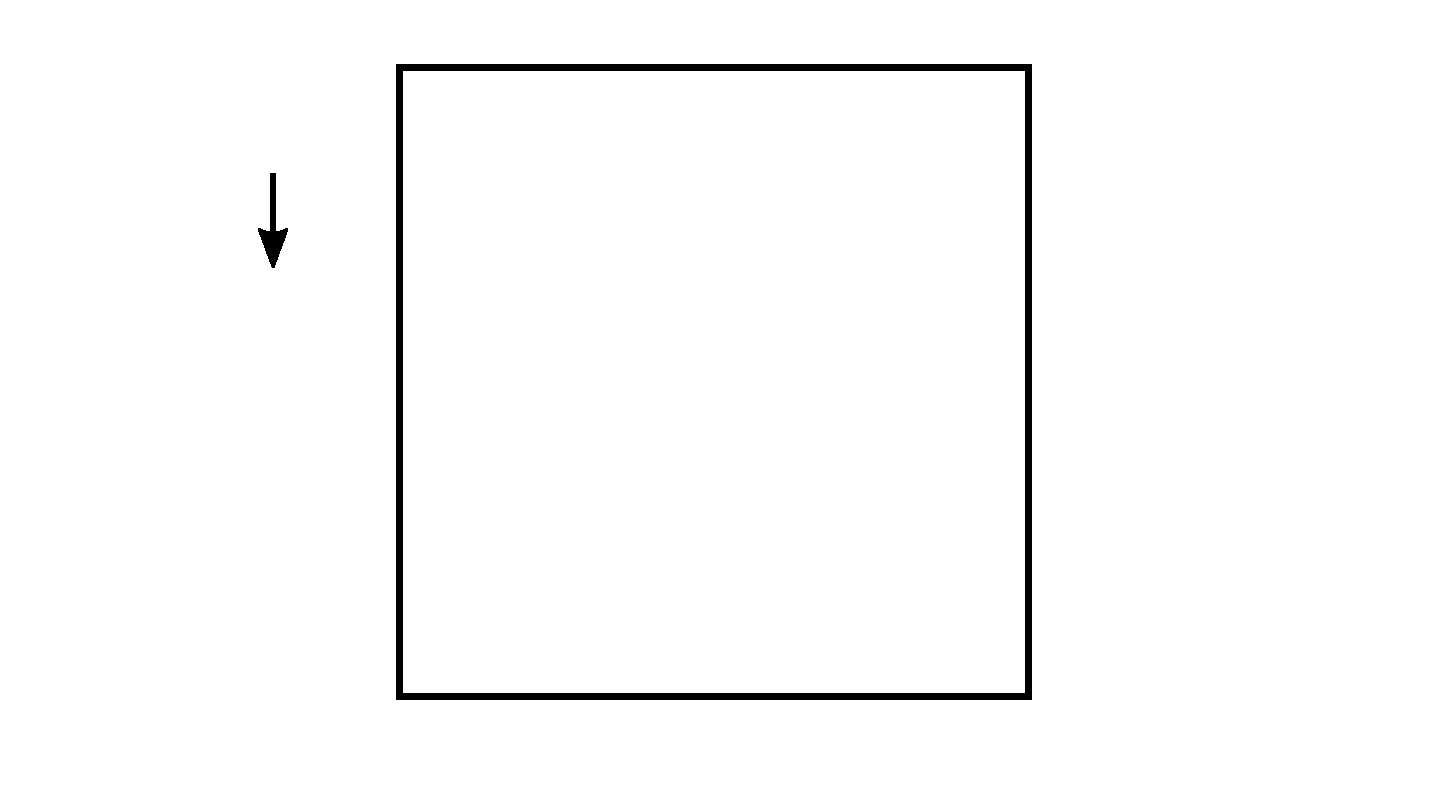
\includegraphics[width=\unitlength,page=1]{../plots/diffheatedCavityGeometry.pdf}}\put(0.49682295,0.08500579){\color[rgb]{0,0,0}\makebox(0,0)[t]{\lineheight{1.25}\smash{\begin{tabular}[t]{c}\text{Adiabatic wall}\end{tabular}}}}\put(0.20516158,0.40737416){\color[rgb]{0,0,0}\makebox(0,0)[lt]{\lineheight{1.25}\smash{\begin{tabular}[t]{l}$g$\end{tabular}}}}\put(0,0){\includegraphics[width=\unitlength,page=2]{../plots/diffheatedCavityGeometry.pdf}}\put(0.49520184,0.44089067){\color[rgb]{0,0,0}\makebox(0,0)[lt]{\lineheight{1.25}\smash{\begin{tabular}[t]{l}$L$\end{tabular}}}}\put(0.66516869,0.28937231){\color[rgb]{0,0,0}\makebox(0,0)[rt]{\lineheight{1.25}\smash{\begin{tabular}[t]{r}$L$\end{tabular}}}}\put(0.27070017,0.28757142){\color[rgb]{0,0,0}\makebox(0,0)[rt]{\lineheight{1.25}\smash{\begin{tabular}[t]{r}$\hat{T}_h$\end{tabular}}}}\put(0.73299485,0.28368869){\color[rgb]{0,0,0}\makebox(0,0)[lt]{\lineheight{1.25}\smash{\begin{tabular}[t]{l}$\hat{T}_c$\end{tabular}}}}\put(0.50040873,0.52453636){\color[rgb]{0,0,0}\makebox(0,0)[t]{\lineheight{1.25}\smash{\begin{tabular}[t]{c}\text{Adiabatic wall}\end{tabular}}}}\put(0,0){\includegraphics[width=\unitlength,page=3]{../plots/diffheatedCavityGeometry.pdf}}\put(0.34544306,0.01736467){\color[rgb]{0,0,0}\makebox(0,0)[lt]{\lineheight{1.25}\smash{\begin{tabular}[t]{l}$x$\end{tabular}}}}\put(0.25242378,0.17511997){\color[rgb]{0,0,0}\makebox(0,0)[lt]{\lineheight{1.25}\smash{\begin{tabular}[t]{l}$y$\end{tabular}}}}\put(0,0){\includegraphics[width=\unitlength,page=4]{../plots/diffheatedCavityGeometry.pdf}}\end{picture}\endgroup \caption{Schematic representation of the differentially heated cavity problem.}
		\label{DHCGeom}
	\end{center}	
\end{figure} 

The differentially heated cavity problem corresponds to a classical benchmark case often used to asses the capability of numerical codes to simulate variable density flows. \cite{paillereComparisonLowMach2000,vierendeelsBenchmarkSolutionsNatural2003,tyliszczakProjectionMethodHighorder2014} In this section, we show the basic set-up and compare our results with the ones presented in the work of Vierendeels et al. \cite{vierendeelsBenchmarkSolutionsNatural2003} where benchmark solutions for the differentially heated cavity are presented. They solve the fully compressible Navier-Stokes equations on a $1024\times1024$ stretched grid using a Finite Volume Method with quadratic convergence.

The differentially heated cavity problem consists of a two-dimensional fully enclosed square cavity filled with fluid.  A sketch of the problem is shown in \cref{DHCGeom}. The left and right walls of the cavity have a constant temperature $\hat{T}_h$ and $\hat{T}_c$ respectively, with $\hat{T}_h >\hat{T}_c$, and the top and bottom walls are adiabatic. A gravity field induces fluid movement due to the density differences caused by the difference of temperature between the hot and cold walls.

The natural convection phenomenon is characterized by the Rayleigh number, defined as 
\begin{equation}\label{eq:Rayleigh}
\text{Ra} = \Prandtl \frac{\hat g \RefVal{\rho}^2(\hat T_h-\hat T_c) \RefVal{L}^3}{\RefVal{T}\RefVal{\mu}^2},
\end{equation}
For small values of $\text{Ra}$, conduction dominates the heat transfer process, and a boundary layer covers the whole domain. On the other hand large values of $\text{Ra}$ represent a convection dominated flow. For increasing $\text{Ra}$ number, a thinner boundary layer is formed. 

\paragraph{Set-up}
A reference velocity for buoyancy driven flows can be defined as\cite{vierendeelsBenchmarkSolutionsNatural2003}
\begin{equation}
\RefVal{u} = \frac{\sqrt{\text{Ra}} \RefVal{\mu}}{\RefVal{\rho}\RefVal{L}}.
\end{equation} 
The Rayleigh number is then related to the Reynolds number according to
\begin{equation}
\text{Re} = \sqrt{\text{Ra}}.
\end{equation}
Thus it is sufficient to select a $\Reynolds$ number in our simulation, fixing the value of the $\text{Ra}$ number. The driving temperature difference $(\hat T_h - \hat T_c)$ appearing in \cref{eq:Rayleigh} can be represented as an non-dimensional parameter:
\begin{equation}\label{eq:nondimensionalTemperature}
\varepsilon = \frac{\hat T_h - \hat T_c}{2\RefVal{T}}.
\end{equation}
Using these definitions, the Froude number can be calculated as 
\begin{equation}
\Froude = \sqrt{\Prandtl 2 \varepsilon}.
\end{equation}
All calculations assume a constant Prandtl number equal to 0.71. The viscosity and heat conductivity  dependence on temperature is calculated using \cref{eq:nondim_sutherland}.
Our results are calculated and compared with those of the reference solution for $\RefVal{T} = 600\si{K}$  and $\varepsilon = 0.6$. The non-dimensional length of the cavity is $L=1$. The non-dimensional temperatures $T_h$ and $T_c$ are set to 1.6 and 0.4, respectively. 
Since the cavity contains a single species, it is governed by the equations for continuity, momentum and temperature (\crefrange{eq:LowMachConti}{eq:LowMachEnergy}) and no equation for species transport is needed. Thus $n_s = 1$ and  $Y_1 = 1$ in the whole domain.  Moreover, the non-dimensional equation of state (\cref{eq:ideal_gas}) only depends on the temperature and reduces to
\begin{equation}
\rho = \frac{p_0}{T}.
\end{equation}
The thermodynamic pressure $p_0$ in a closed system and has to be adapted in order to ensure mass conservation. If $m_0$ is the initial total mass of the system, the thermodynamic pressure is given by
\begin{equation}
p_0 = \frac{m_0}{\int_\Omega \frac{1}{T}\text{d}V}, \label{eq:p0Condition}
\end{equation}
where $\Omega$ represents the complete closed domain. The initial mass of the system $m_0$ is constant and we set $m_0 = 1.0$. Within the solution algorithm, \cref{eq:p0Condition} is used to update the value of the thermodynamic pressure after each Newton-Dogleg iteration.
Moreover, the benchmark solution \cite{vierendeelsBenchmarkSolutionsNatural2003} also reports the Nusselt number and thermodynamic pressure associated with a given Rayleigh number. The Nusselt number is defined for a given wall $\Gamma$ in its averaged form as 
\begin{equation}\label{eq:Nusselt}
\text{Nu}_\Gamma = \frac{1}{T_h - T_c}\int_{\Gamma} k \pfrac{T}{x}\text{d}y.
\end{equation}\begin{table}[t]
	\begin{center}
		\begin{tabular}{cccccc}
			\hline
			Rayleigh & $p_0$ &  $p_{0,\text{ref}}$  &$\text{Nu}_{h}$ & $\text{Nu}_{c}$& $\text{Nu}_{\text{ref}}$ \\ \hline
			\parbox[0pt][13pt][c]{0pt}{}$10^2$   & 0.9574 & 0.9573 & 0.9787    & 0.9787 & 0.9787      \\
			$10^3$   & 0.9381 & 0.9381 & 1.1077    & 1.1077  & 1.1077      \\
			$10^4$   & 0.9146 & 0.9146 & 2.2180    & 2.2174  & 2.2180      \\
			$10^5$   & 0.9220 & 0.9220 & 4.4801    & 4.4796   & 4.4800      \\
			$10^6$   & 0.9245 & 0.9245 & 8.6866    & 8.6791  & 8.6870      \\
			$10^7$   & 0.9225 & 0.9226 & 16.2411   & 16.1700 & 16.2400     \\ \hline
		\end{tabular}
	\end{center}
	\caption[Differentially heated cavity: Results of Nusselt number and Thermodynamic pressure]{Comparison of calculated Nusselt numbers of the hot and cold wall and Thermodynamic pressure $p_0$ reported values\cite{vierendeelsBenchmarkSolutionsNatural2003} for the differentially heated cavity. Results are obtained for polynomial degree of four for the velocities and temperature, three for the pressure in an equidistant $128x128$ mesh.}
	\label{tab:p0_Nu_Results}
\end{table}
\paragraph{Comparison of results with benchmark solution}
The benchmark results \cite{vierendeelsBenchmarkSolutionsNatural2003} are presented for $\text{Ra} = \{10^2,10^3,10^4,10^5,10^6,10^7\}$. In this range of Rayleigh numbers the problem has a steady-state solution, thus we are able to use our steady formulation of the problem. The cavity is represented by the domain $[0,1]\times[0,1]$. We use an equidistant Cartesian mesh with $30 \times 30$ elements for each simulation. A polynomial degree of five is used for the velocities and temperature, and a degree of four for the pressure. 
It is observed that for cases until  $\text{Ra} = 10^5$ the solution of the system using Newton's method is possible without further modifications, while for higher values the algorithm diverges. The homotopy strategy mentioned in \cref{sec:CompMethodology} is used to overcome this problem and obtain solutions for higher Rayleigh (and equivalently higher Reynolds) numbers. Here, the Reynolds number is selected as the homotopy parameter and continuously increased until the desired value is reached.
In \cref{fig:TempProfile,fig:VelocityXProfile,fig:VelocityYProfile} temperature and velocity profiles for different Rayleigh numbers are shown. The profiles calculated with \BoSSS agree closely to the benchmark solution. As expected we observe 
an increase of the acceleration of the fluid in the vicinity of the walls for increasing Rayleigh numbers, forming a thin boundary layer. 



\begin{figure}
	\centering
	\pgfplotsset{width=0.45 \textwidth, compat=1.3}
	\begin{tikzpicture}
	\begin{groupplot}[
	group style={group size=2 by 3,		
		horizontal sep = 1.5cm,
		vertical sep = 2.0cm,
		xlabels at=edge bottom,
		ylabels at=edge left,
	},
	axis on top,
	scale only axis,
	enlargelimits=false,	
	axis equal image,
	xlabel = $x$,
	ylabel = $y$,
	xtick = {0.0, 0.5, 1},
	ytick = {0.0, 0.5, 1},
	]
	\nextgroupplot[title = {$ \gls{Reynolds}= 10^2$}]
	\addplot[thick,blue] graphics[	xmin=0,	xmax=1.0,	ymin=0.0,	ymax=1.0,] {../plots/HSC_streamline.0000.png};
	\nextgroupplot[title = {$ \gls{Reynolds}= 10^3$}]
	\addplot[thick,blue] graphics[	xmin=0,	xmax=1.0,	ymin=0.0,	ymax=1.0,]  {../plots/HSC_streamline.0001.png};
	\nextgroupplot[title = {$ \gls{Reynolds}= 10^4$}]
	\addplot[thick,blue] graphics[	xmin=0,	xmax=1.0,	ymin=0.0,	ymax=1.0,]  {../plots/HSC_streamline.0002.png};
	\nextgroupplot[title = {$ \gls{Reynolds}= 10^5$}]
	\addplot[thick,blue] graphics[	xmin=0,	xmax=1.0,	ymin=0.0,	ymax=1.0,]  {../plots/HSC_streamline.0003.png};
	\nextgroupplot[title = {$ \gls{Reynolds}= 10^6$}]
	\addplot[thick,blue] graphics[xmin=0,	xmax=1.0,	ymin=0.0,	ymax=1.0,]  {../plots/HSC_streamline.0004.png};
	\nextgroupplot[title = {$ \gls{Reynolds}= 10^7$}]
	\addplot[thick,blue] graphics[xmin=0,	xmax=1.0,	ymin=0.0,	ymax=1.0,]  {../plots/HSC_streamline.0005.png};
	\end{groupplot}	
	\end{tikzpicture}
	\caption{Streamlines of the heated cavity configuration with $\epsilon = 0.6$.}
\end{figure}


\begin{figure}[!htb]
	\centering
	\pgfplotsset{width=0.20\textwidth, compat=1.3}
	\begin{tikzpicture}
	\begin{groupplot}[
	group style={
		group name= group,
		group size=3 by 2,
		horizontal sep = 2.0cm,
		vertical sep = 2.0cm,
	},
	xmin=0, xmax=1.0,
	ymin=-0.4, ymax = 0.4,
	x tick label style={
		/pgf/number format/.cd,
		precision=3,
		/tikz/.cd
	},
	xlabel=$y$,
	ylabel= $u_x$,
	xmajorgrids,
	ymajorgrids,
	legend style={at={(1,1)}, anchor=north east},
	]
	\nextgroupplot[title = {$\text{Ra} = 10^2$}]
	\addplot+[color=black, no marks] table {data/HeatedSquareCavity_VelocityXComparison/VelocityX0.txt};
	\addplot+[color=black, only marks] table {data/HeatedSquareCavity_VelocityXComparison/VelocityX0_REF.txt};
	\nextgroupplot[title = {$\text{Ra} = 10^3$}]
	\addplot+[color=black, no marks] table {data/HeatedSquareCavity_VelocityXComparison/VelocityX1.txt};
	\addplot+[color=black, only marks] table {data/HeatedSquareCavity_VelocityXComparison/VelocityX1_REF.txt};
	\nextgroupplot[title = {$\text{Ra} = 10^4$}]
	\addplot+[color=black, no marks] table {data/HeatedSquareCavity_VelocityXComparison/VelocityX2.txt};
	\addplot+[color=black, only marks] table {data/HeatedSquareCavity_VelocityXComparison/VelocityX2_REF.txt};
	\nextgroupplot[title = {$\text{Ra} = 10^5$}]
	\addplot+[color=black, no marks] table {data/HeatedSquareCavity_VelocityXComparison/VelocityX3.txt};
	\addplot+[color=black, only marks] table {data/HeatedSquareCavity_VelocityXComparison/VelocityX3_REF.txt};
	\nextgroupplot[title = {$\text{Ra} = 10^6$}]
	\addplot+[color=black, no marks] table {data/HeatedSquareCavity_VelocityXComparison/VelocityX4.txt};
	\addplot+[color=black, only marks] table {data/HeatedSquareCavity_VelocityXComparison/VelocityX4_REF.txt};
	\nextgroupplot[title = {$\text{Ra} = 10^7$}]
	\addplot+[color=black, no marks] table {data/HeatedSquareCavity_VelocityXComparison/VelocityX5.txt};
	\addplot+[color=black, only marks] table {data/HeatedSquareCavity_VelocityXComparison/VelocityX5_REF.txt};
	\end{groupplot}
	\end{tikzpicture}
	\caption{ Profiles of the x-velocity component along the vertical line $x=0.5$. Solid lines represents our solution and the marks the benchmark solution. \cite{vierendeelsBenchmarkSolutionsNatural2003}}
	\label{fig:VelocityXProfile}
\end{figure}


\begin{figure}[b!]
	\centering
	\pgfplotsset{width=0.20\textwidth, compat=1.3}
	\begin{tikzpicture}
	\begin{groupplot}[
	group style={
		group name= group,
		group size=3 by 2,
		horizontal sep = 2.0cm,
		vertical sep = 2.0cm,
	},
	xmin=0, xmax=1.0,
	ymin=-0.4, ymax=0.4,
	x tick label style={
		/pgf/number format/.cd,
		precision=3,
		/tikz/.cd
	},
	xlabel=$x$,
	ylabel= $u_y$,
	xmajorgrids,
	ymajorgrids,
	legend style={at={(1,1)}, anchor=north east},
	]
	\nextgroupplot[title = {$\text{Ra} = 10^2$}]
	\addplot+[color=black, no marks] table {data/HeatedSquareCavity_VelocityYComparison/VelocityY0.txt};
	\addplot+[color=black, only marks] table {data/HeatedSquareCavity_VelocityYComparison/VelocityY0_REF.txt};
	\nextgroupplot[title = {$\text{Ra} = 10^3$}]
	\addplot+[color=black, no marks] table {data/HeatedSquareCavity_VelocityYComparison/VelocityY1.txt};
	\addplot+[color=black, only marks] table {data/HeatedSquareCavity_VelocityYComparison/VelocityY1_REF.txt};
	\nextgroupplot[title = {$\text{Ra} = 10^4$}]
	\addplot+[color=black, no marks] table {data/HeatedSquareCavity_VelocityYComparison/VelocityY2.txt};
	\addplot+[color=black, only marks] table {data/HeatedSquareCavity_VelocityYComparison/VelocityY2_REF.txt};
	\nextgroupplot[title = {$\text{Ra} = 10^5$}]
	\addplot+[color=black, no marks] table {data/HeatedSquareCavity_VelocityYComparison/VelocityY3.txt};
	\addplot+[color=black, only marks] table {data/HeatedSquareCavity_VelocityYComparison/VelocityY3_REF.txt};
	\nextgroupplot[title = {$\text{Ra} = 10^6$}]
	\addplot+[color=black, no marks] table {data/HeatedSquareCavity_VelocityYComparison/VelocityY4.txt};
	\addplot+[color=black, only marks] table {data/HeatedSquareCavity_VelocityYComparison/VelocityY4_REF.txt};
	\nextgroupplot[title = {$\text{Ra} = 10^7$}]
	\addplot+[color=black, no marks] table {data/HeatedSquareCavity_VelocityYComparison/VelocityY5.txt};
	\addplot+[color=black, only marks] table {data/HeatedSquareCavity_VelocityYComparison/VelocityY5_REF.txt};
	\end{groupplot}
	\end{tikzpicture}
	\caption{ Profiles of the y-velocity component along the horizontal line $y=0.5$. Solid lines represents our solution and marks the benchmark solution. \cite{vierendeelsBenchmarkSolutionsNatural2003}}
	\label{fig:VelocityYProfile}
\end{figure}
We also compare the thermodynamic pressure and the Nusselt numbers to the benchmark solution. The results are shown in \cref{tab:p0_Nu_Results}. The thermodynamic pressure is obtained from \cref{eq:p0Condition}, and the Nusselt number is calculated with \cref{eq:Nusselt}. We observe that our results are in very good agreement with the reference results, and the thermodynamic pressure differ at most in the fourth decimal place. Note that the Nusselt number of the heated  wall $(\text{Nu}_\text{h})$ and the Nusselt number of the cold wall $(\text{Nu}_\text{c})$ are different.  As the Rayleigh number grows, this discrepancy becomes bigger, hinting that at such Rayleigh numbers the used mesh is not refined enough  to represent adequately the thin boundary layer and more complex flow structures appearing at high-Rayleigh cases. While for an energy conservative system $\text{Nu}_\text{h}$ and $\text{Nu}_c$ should be equal, for our formulation this is not the case and the values differ slightly. This discrepancy can be seen as a measure of the discretization error from the DG formulation.\cite{kleinHighorderDiscontinuousGalerkin2016} This hints that the discrepancy between Nusselt numbers should decrease when increasing the mesh resolution, which will be discussed in the next section. 


\begin{figure}[b!]
	\centering
	\pgfplotsset{width=0.20\textwidth, compat=1.3}
	\begin{tikzpicture}
	\begin{groupplot}[
	group style={
		group name= group,
		group size=3 by 2,
		horizontal sep = 2.0cm,
		vertical sep = 2.0cm,
	},
	xmin=0, xmax=1.0,
	ymin=0.4, ymax =1.6, 
	x tick label style={
		/pgf/number format/.cd,
		precision=3,
		/tikz/.cd
	},
	xlabel=$x$,
	ylabel= T,
	xmajorgrids,
	ymajorgrids,
	legend style={at={(0,0)}, anchor=south west},
	]
	\nextgroupplot[title = {$\text{Ra} = 10^2$}]
	\addplot[solid,every mark/.append style={solid, fill=gray}, mark=triangle*] coordinates{(-1,-1)};
	\addplot[dashed,every mark/.append style={solid, fill=gray}, mark=diamond*] coordinates{(-1,-1)};
	\addplot[densely dashdotted,every mark/.append style={solid, fill=gray}, mark=oplus*] coordinates{(-1,-1)};
	\addlegendentry{$y = 0$};
	\addlegendentry{$y = 0.5$};
	\addlegendentry{$y = 1$};
	\addplot+[color=black, only marks] table {data/HeatedSquareCavity_TemperatureComparison/Temperatures_bot_Ra0_REF.txt};
	\addplot+[color=black, only marks] table {data/HeatedSquareCavity_TemperatureComparison/Temperatures_mid_Ra0_REF.txt};
	\addplot+[color=black, only marks] table {data/HeatedSquareCavity_TemperatureComparison/Temperatures_top_Ra0_REF.txt};
	\addplot+[color=black, no marks] table {data/HeatedSquareCavity_TemperatureComparison/Temperatures_bot_Ra0.txt};
	\addplot+[color=black, no marks] table {data/HeatedSquareCavity_TemperatureComparison/Temperatures_mid_Ra0.txt};
	\addplot+[color=black, no marks] table {data/HeatedSquareCavity_TemperatureComparison/Temperatures_top_Ra0.txt};
	\nextgroupplot[title = {$\text{Ra} = 10^3$}]
	\addplot+[color=black, no marks] table {data/HeatedSquareCavity_TemperatureComparison/Temperatures_bot_Ra1.txt};
	\addplot+[color=black, no marks] table {data/HeatedSquareCavity_TemperatureComparison/Temperatures_mid_Ra1.txt};
	\addplot+[color=black, no marks] table {data/HeatedSquareCavity_TemperatureComparison/Temperatures_top_Ra1.txt};
	\addplot+[color=black, only marks] table {data/HeatedSquareCavity_TemperatureComparison/Temperatures_bot_Ra1_REF.txt};
	\addplot+[color=black, only marks] table {data/HeatedSquareCavity_TemperatureComparison/Temperatures_mid_Ra1_REF.txt};
	\addplot+[color=black, only marks] table {data/HeatedSquareCavity_TemperatureComparison/Temperatures_top_Ra1_REF.txt};
	\nextgroupplot[title = {$\text{Ra} = 10^4$}]
	\addplot+[color=black, no marks] table {data/HeatedSquareCavity_TemperatureComparison/Temperatures_bot_Ra2.txt};
	\addplot+[color=black, no marks] table {data/HeatedSquareCavity_TemperatureComparison/Temperatures_mid_Ra2.txt};
	\addplot+[color=black, no marks] table {data/HeatedSquareCavity_TemperatureComparison/Temperatures_top_Ra2.txt};
	\addplot+[color=black, only marks] table {data/HeatedSquareCavity_TemperatureComparison/Temperatures_bot_Ra2_REF.txt};
	\addplot+[color=black, only marks] table {data/HeatedSquareCavity_TemperatureComparison/Temperatures_mid_Ra2_REF.txt};
	\addplot+[color=black, only marks] table {data/HeatedSquareCavity_TemperatureComparison/Temperatures_top_Ra2_REF.txt};
	\nextgroupplot[title = {$\text{Ra} = 10^5$}]
	\addplot+[color=black, no marks] table {data/HeatedSquareCavity_TemperatureComparison/Temperatures_bot_Ra3.txt};
	\addplot+[color=black, no marks] table {data/HeatedSquareCavity_TemperatureComparison/Temperatures_mid_Ra3.txt};
	\addplot+[color=black, no marks] table {data/HeatedSquareCavity_TemperatureComparison/Temperatures_top_Ra3.txt};
	\addplot+[color=black, only marks] table {data/HeatedSquareCavity_TemperatureComparison/Temperatures_bot_Ra3_REF.txt};
	\addplot+[color=black, only marks] table {data/HeatedSquareCavity_TemperatureComparison/Temperatures_mid_Ra3_REF.txt};
	\addplot+[color=black, only marks] table {data/HeatedSquareCavity_TemperatureComparison/Temperatures_top_Ra3_REF.txt};
	\nextgroupplot[title = {$\text{Ra} = 10^6$}]
	\addplot+[color=black, no marks] table {data/HeatedSquareCavity_TemperatureComparison/Temperatures_bot_Ra4.txt};
	\addplot+[color=black, no marks] table {data/HeatedSquareCavity_TemperatureComparison/Temperatures_mid_Ra4.txt};
	\addplot+[color=black, no marks] table {data/HeatedSquareCavity_TemperatureComparison/Temperatures_top_Ra4.txt};
	\addplot+[color=black, only marks] table {data/HeatedSquareCavity_TemperatureComparison/Temperatures_bot_Ra4_REF.txt};
	\addplot+[color=black, only marks] table {data/HeatedSquareCavity_TemperatureComparison/Temperatures_mid_Ra4_REF.txt};
	\addplot+[color=black, only marks] table {data/HeatedSquareCavity_TemperatureComparison/Temperatures_top_Ra4_REF.txt};
	\nextgroupplot[title = {$\text{Ra} = 10^7$}]
	\addplot+[color=black, no marks] table {data/HeatedSquareCavity_TemperatureComparison/Temperatures_bot_Ra5.txt};
	\addplot+[color=black, no marks] table {data/HeatedSquareCavity_TemperatureComparison/Temperatures_mid_Ra5.txt};
	\addplot+[color=black, no marks] table {data/HeatedSquareCavity_TemperatureComparison/Temperatures_top_Ra5.txt};
	\addplot+[color=black, only marks] table {data/HeatedSquareCavity_TemperatureComparison/Temperatures_bot_Ra5_REF.txt};
	\addplot+[color=black, only marks] table {data/HeatedSquareCavity_TemperatureComparison/Temperatures_mid_Ra5_REF.txt};
	\addplot+[color=black, only marks] table {data/HeatedSquareCavity_TemperatureComparison/Temperatures_top_Ra5_REF.txt};
	\end{groupplot}
	\end{tikzpicture}
	\caption{Temperature profiles for the differentially heated square cavity along different vertical levels. Solid lines represent our solution and marks the benchmark solution. \cite{vierendeelsBenchmarkSolutionsNatural2003}}
	\label{fig:TempProfile}
\end{figure}

\begin{figure}[b!]
	\centering
	\begin{tikzpicture}
	\begin{groupplot}[
	group style={
		group name= group,
		group size=3 by 2,
		xlabels at=edge bottom,
		ylabels at=edge left,
		horizontal sep = 2.0cm,
		vertical sep = 1.5cm,
	},
	grid = major,
	width=3.5cm,
	height=3.5cm,
	xlabel= $\sqrt{\text{Number of cells}}$,
	ylabel= Nusselt,
	xtick=data,
	max space between ticks=1000pt,
	try min ticks=5,
	y tick label style= {
		/pgf/number format/.cd,
		fixed,
		fixed zerofill,
		precision = 4,
		legend style = {at={(1,0)},anchor = south east}
	}
	]
	\nextgroupplot[title = {$\mathbf{Ra = 10^2, k = 2}$}]
	\addplot [solid,mark = *, ]  table {data/NusseltStudy/NusseltReLeft100Dg2.txt};
	\addlegendentry{$\text{Nu}_h$};
	\addplot [solid, mark = square, ] table {data/NusseltStudy/NusseltReRight100Dg2.txt};
	\addlegendentry{$\text{Nu}_c$};
	\addplot [dashed, very thick] table {data/NusseltStudy/ReferenceNusselt100Dg2.txt};	
	\addlegendentry{$\text{Nu}_{\text{ref}}$};	
	\nextgroupplot[title = {$\mathbf{Ra = 10^2, k = 3}$}]
	\addplot [solid,mark = *, ] table {data/NusseltStudy/NusseltReLeft100Dg3.txt};	
	\addlegendentry{$\text{Nu}_h$};
	\addplot [solid, mark = square,] table {data/NusseltStudy/NusseltReRight100Dg3.txt};
	\addlegendentry{$\text{Nu}_c$};
	\addplot [dashed, very thick] table {data/NusseltStudy/ReferenceNusselt100Dg3.txt};	
	\addlegendentry{$\text{Nu}_{\text{ref}}$};		
	\nextgroupplot[title = {$\mathbf{Ra = 10^2, k = 4}$}]
	\addplot [solid,mark = *, ] table {data/NusseltStudy/NusseltReLeft100Dg4.txt};	
	\addlegendentry{$\text{Nu}_h$};
	\addplot [solid, mark = square,] table {data/NusseltStudy/NusseltReRight100Dg4.txt};	
	\addlegendentry{$\text{Nu}_c$};
	\addplot [dashed, very thick] table {data/NusseltStudy/ReferenceNusselt100Dg4.txt};	
	\addlegendentry{$\text{Nu}_{\text{ref}}$};
	\nextgroupplot[title = {$\mathbf{Ra = 10^6, k = 2}$},ymax=9]
	\addplot [solid,mark = *,]  table {data/NusseltStudy/NusseltReLeft1000000Dg2.txt};	
	\addlegendentry{$\text{Nu}_h$};
	\addplot [solid, mark = square, ] table {data/NusseltStudy/NusseltReRight1000000Dg2.txt};	
	\addlegendentry{$\text{Nu}_c$};
	\addplot [dashed, very thick] table {data/NusseltStudy/ReferenceNusselt1000000Dg2.txt};	
	\addlegendentry{$\text{Nu}_{\text{ref}}$};
	\nextgroupplot[title = {$\mathbf{Ra = 10^6, k = 3}$}]
	\addplot [solid,mark = *, ] table {data/NusseltStudy/NusseltReLeft1000000Dg3.txt};	
	\addlegendentry{$\text{Nu}_h$};
	\addplot [solid, mark = square, ] table {data/NusseltStudy/NusseltReRight1000000Dg3.txt};	
	\addlegendentry{$\text{Nu}_c$};
	\addplot [dashed, very thick] table {data/NusseltStudy/ReferenceNusselt1000000Dg3.txt};	
	\addlegendentry{$\text{Nu}_{\text{ref}}$};
	\nextgroupplot[title = {$\mathbf{Ra = 10^6, k = 4}$}]
	\addplot [solid,mark = *, ] table {data/NusseltStudy/NusseltReLeft1000000Dg4.txt};	
	\addlegendentry{$\text{Nu}_h$};
	\addplot [solid, mark = square, ] table {data/NusseltStudy/NusseltReRight1000000Dg4.txt};	
	\addlegendentry{$\text{Nu}_c$};
	\addplot [dashed, very thick] table {data/NusseltStudy/ReferenceNusselt1000000Dg4.txt};	
	\addlegendentry{$\text{Nu}_{\text{ref}}$};
	\end{groupplot}
	\end{tikzpicture}
	\caption{Nusselt numbers calculated with \cref{eq:Nusselt} at the hot wall ($\text{Nu}_h$) and the cold wall ($\text{Nu}_c$) for different number of cells and polynomial order $k$. The reference values\cite{vierendeelsBenchmarkSolutionsNatural2003} are shown with dashed lines.}\label{fig:NusseltStudy}
\end{figure}

\paragraph{Convergence study}\label{ssec:ConvStudyHeatedCavity}
An $h-$convergence study of the differentially heated cavity configuration was conducted. Calculations were done for polynomial degrees $k = {1,2,3,4}$ and equidistant regular meshes with respectively $8, 16, 32, 64, 128$ and $256$ elements in each spatial coordinate.  The $L^2$-Norm was used for the calculation of the errors against the solution on the finest mesh. Results of the $h$-convergence study for varying polynomial orders $k$ are shown in \cref{fig:ConvergenceDHC}. Recall that for increasing polynomial order, the expected order of convergence is given by the slope of the line curve when cell length and errors are presented in a log-log plot. Because we are using a mixed order formulation the slopes should be equal to $k$ for the pressure and equal to $k+1$ for all other variables.  It is observed how convergence rates scale approximately as $k+1$. Interestingly, for $k=2$ the rates are higher than expected. On the other hand, some degeneration on the convergence rates is observed for $k = 4$.

As discussed in the last section, the difference on values of the Nusselt number on the hot wall $\text{Nu}_\text{h}$ and the cold wall $\text{Nu}_c$ is a consequence of spatial discretization error. In \cref{fig:NusseltStudy} the convergence behaviour of the Nusselt number for different polynomial degrees $k$, different number of elements and for two different Ra numbers is presented. As expected, it can be observed that this discrepancy is smaller when a higher number of elements is used. 


\begin{figure}[t!]
	\centering
	\pgfplotsset{width=0.34\textwidth, compat=1.3}
	\begin{tikzpicture}
	\begin{groupplot}[
	group style={
		group name= group,
		group size=2 by 2,
		ylabels at=edge left,
		horizontal sep = 2.5cm,
		vertical sep = 1.5cm,
	},
	xtick={2^-8,2^-7,2^-6, 2^-5, 2^-4,2^-3},
	xticklabels = {$2^{-8}$,$2^{-7}$,$2^{-6}$,$2^{-5}$, $2^{-4}$, $2^{-3}$},
	xlabel=Cell length $h$,
	xmajorgrids,
	ymajorgrids,
	legend style={at={(1,0)}, anchor=south east},
	]
	\nextgroupplot[xmode=log, ymode=log,ylabel = $\LtwoNorm{ u_x - u_{x,\text{fine}}}$,]
	\addplot+[color=black, dashed] table {data/HSC_convstudy_XNSEC/VelocityXDG1Data.txt};
	\addlegendentry{$k=1$};
	\addplot[solid,  forget plot] table [   
	x=x,
	y={create col/linear regression={y=y,
			variance list={10000,800,600,500,400,200,100}}}]
	{data/HSC_convstudy_XNSEC/VelocityXDG1Data.txt}
	coordinate [pos=0.75] (A)
	coordinate [pos=0.90] (B)
	;
	\xdef\slopeXA{\pgfplotstableregressiona}			
	\draw (A) |- (B)
	node [pos=0.55,anchor= west]
	{\pgfmathprintnumber{\slopeXA}};			
	\addplot+[color=black, dashed] table {data/HSC_convstudy_XNSEC/VelocityXDG2Data.txt};
	\addlegendentry{$k=2$};
	\addplot[solid, forget plot] table [   
	x=x,
	y={create col/linear regression={y=y,
			variance list={10000,800,600,500,400,200,100}				
	}}]
	{data/HSC_convstudy_XNSEC/VelocityXDG2Data.txt}
	coordinate [pos=0.75] (A)
	coordinate [pos=0.90] (B)
	;
	\xdef\slopeXB{\pgfplotstableregressiona}			
	\draw (A) |- (B)
	node [pos=0.15,anchor=  west]
	{\pgfmathprintnumber{\slopeXB}};			
	\addplot+[color=black, dashed] table {data/HSC_convstudy_XNSEC/VelocityXDG3Data.txt};
	\addlegendentry{$k=3$};			
	\addplot[solid, forget plot] table [   
	x=x,
	y={create col/linear regression={y=y,
			variance list={10000,800,600,500,400,200,100}}}]
	{data/HSC_convstudy_XNSEC/VelocityXDG3Data.txt}
	coordinate [pos=0.80] (A)
	coordinate [pos=0.95] (B)
	;
	\xdef\slopeXC{\pgfplotstableregressiona}			
	\draw (A) |- (B)
	node [pos=0,anchor=east]
	{\pgfmathprintnumber{\slopeXC}};			
	\addplot+[color=black, dashed] table {data/HSC_convstudy_XNSEC/VelocityXDG4Data.txt};
	\addlegendentry{$k=4$};
	\addplot[solid, forget plot] table [   
	x=x,
	y={create col/linear regression={y=y,
			variance list={10000,800,600,500,400,200,100}}}]
	{data/HSC_convstudy_XNSEC/VelocityXDG4Data.txt}
	coordinate [pos=0.75] (A)
	coordinate [pos=0.9] (B)
	;
	\xdef\slopeXD{\pgfplotstableregressiona}			
	\draw (A) |- (B)
	node [pos=0.55,anchor=south west]
	{\pgfmathprintnumber{\slopeXD}};	
	\nextgroupplot[xmode=log, ymode=log,	ylabel = $\LtwoNorm{ u_y - u_{y,\text{fine}}}$,]
	\addplot+[color=black, dashed] table {data/HSC_convstudy_XNSEC/VelocityYDG1Data.txt};
	\addlegendentry{$k=1$};
	\addplot[solid,  forget plot] table [   
	x=x,
	y={create col/linear regression={y=y,
			variance list={10000,800,600,500,400,200,100}}}]
	{data/HSC_convstudy_XNSEC/VelocityYDG1Data.txt}
	coordinate [pos=0.75] (A)
	coordinate [pos=0.90] (B)
	;
	\xdef\slopeXA{\pgfplotstableregressiona}			
	\draw (A) |- (B)
	node [pos=0.55,anchor= west]
	{\pgfmathprintnumber{\slopeXA}};			
	\addplot+[color=black, dashed] table {data/HSC_convstudy_XNSEC/VelocityYDG2Data.txt};
	\addlegendentry{$k=2$};
	\addplot[solid, forget plot] table [   
	x=x,
	y={create col/linear regression={y=y,
			variance list={10000,800,600,500,400,200,100}}}]
	{data/HSC_convstudy_XNSEC/VelocityYDG2Data.txt}
	coordinate [pos=0.75] (A)
	coordinate [pos=0.90] (B)
	;
	\xdef\slopeXB{\pgfplotstableregressiona}			
	\draw (A) |- (B)
	node [pos=0.55,anchor=  west]
	{\pgfmathprintnumber{\slopeXB}};			
	\addplot+[color=black, dashed] table {data/HSC_convstudy_XNSEC/VelocityYDG3Data.txt};
	\addlegendentry{$k=3$};			
	\addplot[solid, forget plot] table [   
	x=x,
	y={create col/linear regression={y=y,
			variance list={10000,800,600,500,400,200,100}}}]
	{data/HSC_convstudy_XNSEC/VelocityYDG3Data.txt}
	coordinate [pos=0.75] (A)
	coordinate [pos=0.90] (B)
	;
	\xdef\slopeXC{\pgfplotstableregressiona}			
	\draw (A) |- (B)
	node [pos=0.55,anchor=south west]
	{\pgfmathprintnumber{\slopeXC}};			
	\addplot+[color=black, dashed] table {data/HSC_convstudy_XNSEC/VelocityYDG4Data.txt};
	\addlegendentry{$k=4$};
	\addplot[solid, forget plot] table [   
	x=x,
	y={create col/linear regression={y=y,
			variance list={10000,800,600,500,400,200,100}}}]
	{data/HSC_convstudy_XNSEC/VelocityYDG4Data.txt}
	coordinate [pos=0.75] (A)
	coordinate [pos=0.9] (B)
	;
	\xdef\slopeXD{\pgfplotstableregressiona}			
	\draw (A) |- (B)
	node [pos=0.55,anchor=south west]
	{\pgfmathprintnumber{\slopeXD}};	
	\nextgroupplot[ xmode=log, ymode=log,	ylabel=$ \LtwoNorm{T - T_{\text{fine}}}$,]
	\addplot+[color=black, dashed] table {data/HSC_convstudy_XNSEC/TemperatureDG1Data.txt};
	\addlegendentry{$k=1$};
	\addplot[solid,  forget plot] table [   
	x=x,
	y={create col/linear regression={y=y,
			variance list={10000,800,600,500,400,200,100}}}]
	{data/HSC_convstudy_XNSEC/TemperatureDG1Data.txt}
	coordinate [pos=0.75] (A)
	coordinate [pos=0.90] (B)
	;
	\xdef\slopeXA{\pgfplotstableregressiona}			
	\draw (A) |- (B)
	node [pos=0.55,anchor= west]
	{\pgfmathprintnumber{\slopeXA}};			
	\addplot+[color=black, dashed] table {data/HSC_convstudy_XNSEC/TemperatureDG2Data.txt};
	\addlegendentry{$k=2$};
	\addplot[solid, forget plot] table [   
	x=x,
	y={create col/linear regression={y=y,
			variance list={10000,800,600,500,400,200,100}}}]
	{data/HSC_convstudy_XNSEC/TemperatureDG2Data.txt}
	coordinate [pos=0.75] (A)
	coordinate [pos=0.85] (B)
	;
	\xdef\slopeXB{\pgfplotstableregressiona}			
	\draw (A) |- (B)
	node [pos=0.55,anchor=  west]
	{\pgfmathprintnumber{\slopeXB}};			
	\addplot+[color=black, dashed] table {data/HSC_convstudy_XNSEC/TemperatureDG3Data.txt};
	\addlegendentry{$k=3$};			
	\addplot[solid, forget plot] table [   
	x=x,
	y={create col/linear regression={y=y,
			variance list={10000,800,600,500,400,200,100}}}]
	{data/HSC_convstudy_XNSEC/TemperatureDG3Data.txt}
	coordinate [pos=0.75] (A)
	coordinate [pos=0.90] (B)
	;
	\xdef\slopeXC{\pgfplotstableregressiona}			
	\draw (A) |- (B)
	node [pos=0.55,anchor=south west]
	{\pgfmathprintnumber{\slopeXC}};			
	\addplot+[color=black, dashed] table {data/HSC_convstudy_XNSEC/TemperatureDG4Data.txt};
	\addlegendentry{$k=4$};
	\addplot[solid, forget plot] table [   
	x=x,
	y={create col/linear regression={y=y,
			variance list={100000,800000,600,500,400,200,100}}}]
	{data/HSC_convstudy_XNSEC/TemperatureDG4Data.txt}
	coordinate [pos=0.75] (A)
	coordinate [pos=0.9] (B)
	;
	\xdef\slopeXD{\pgfplotstableregressiona}			
	\draw (A) |- (B)
	node [pos=0.55,anchor=south west]
	{\pgfmathprintnumber{\slopeXD}};
	\nextgroupplot[xmode=log, ymode=log,ylabel=$\LtwoNorm{ p - p_{\text{fine}} }$,]
	\addplot+[color=black, dashed] table {data/HSC_convstudy_XNSEC/PressureDG1Data.txt};
	\addlegendentry{$k'=0$};
	\addplot[solid,  forget plot] table [   
	x=x,
	y={create col/linear regression={y=y,
			variance list={10000,800,600,500,400,200,100}}}]
	{data/HSC_convstudy_XNSEC/PressureDG1Data.txt}
	coordinate [pos=0.75] (A)
	coordinate [pos=0.90] (B)
	;
	\xdef\slopeXA{\pgfplotstableregressiona}			
	\draw (A) |- (B)
	node [pos=0.55,anchor= west]
	{\pgfmathprintnumber{\slopeXA}};			
	\addplot+[color=black, dashed] table {data/HSC_convstudy_XNSEC/PressureDG2Data.txt};
	\addlegendentry{$k'=1$};
	\addplot[solid, forget plot] table [   
	x=x,
	y={create col/linear regression={y=y,
			variance list={10000,800,600,500,400,200,100}}}]
	{data/HSC_convstudy_XNSEC/PressureDG2Data.txt}
	coordinate [pos=0.80] (A)
	coordinate [pos=0.95] (B)
	;
	\xdef\slopeXB{\pgfplotstableregressiona}			
	\draw (A) |- (B)
	node [pos=0, anchor =east]
	{\pgfmathprintnumber{\slopeXB}};			
	\addplot+[color=black, dashed] table {data/HSC_convstudy_XNSEC/PressureDG3Data.txt};
	\addlegendentry{$k'=2$};			
	\addplot[solid, forget plot] table [   
	x=x,
	y={create col/linear regression={y=y,
			variance list={10000,800,600,500,400,200,100}}}]
	{data/HSC_convstudy_XNSEC/PressureDG3Data.txt}
	coordinate [pos=0.75] (A)
	coordinate [pos=0.90] (B)
	;
	\xdef\slopeXC{\pgfplotstableregressiona}			
	\draw (A) |- (B)
	node [pos=0.55,anchor=south west]
	{\pgfmathprintnumber{\slopeXC}};			
	\addplot+[color=black, dashed] table {data/HSC_convstudy_XNSEC/PressureDG4Data.txt};
	\addlegendentry{$k'=3$};
	\addplot[solid, forget plot] table [   
	x=x,
	y={create col/linear regression={y=y,
			variance list={10000,800,600,500,400,200,100}}}]
	{data/HSC_convstudy_XNSEC/PressureDG4Data.txt}
	coordinate [pos=0.75] (A)
	coordinate [pos=0.9] (B)
	;
	\xdef\slopeXD{\pgfplotstableregressiona}			
	\draw (A) |- (B)
	node [pos=0.55,anchor=south west]
	{\pgfmathprintnumber{\slopeXD}};		
	\end{groupplot}
	\end{tikzpicture}
	\caption{Convergence study of the differentially heated cavity problem for $\text{Ra} = 10^3$.}\label{fig:ConvergenceDHC}
\end{figure}




\subsection{Poiseuille–Rayleigh–Bénard instability in a channel}
\blindtext[5]


\subsection{Flow around a heated cylinder}
\subsubsection{Square cylinder}
\blindtext[5]
\subsubsection{Circle? cylinder}
\blindtext[5]



\section{Multi-component non-isothermal cases}
In the following, we show results of the simulations of two test cases with combustion, namely the counterflow diffusion flame and the chambered diffusion flame. For both cases, the solution of the flame sheet problem described in \cref{ssec:FlameSheet} is calculated first. This solution is used subsequently as initial estimates for the solution of the finite chemistry rate problem (c.f. \cref{ssec:NonDimLowMachEquations}). In all test cases presented in this section, a smoothing parameter $\sigma = 50$ was used (c.f. \cref{ssec:FlameSheet}). For all test cases methane combustion according to the one-step model shown in \cref{sec:ChemModel} is considered. The mass fraction transport \cref{eq:LowMachMassBalance} is solved for the species \ch{CH4}, \ch{O2}, \ch{CO2} and \ch{H2O}, thus $\vec{Y}' = \left(Y_{\ch{CH4}},Y_{\ch{O2}},Y_{\ch{CO2}},Y_{\ch{H2O}}\right)$. The nitrogen mass fraction $Y_{\ch{N2}}$ is calculated according to \cref{eq:MassFractionConstraint}. 



\subsection{CoFlowing flame?}

As a first test for assessing basic behaviour related to combustion, a cofloing flame configuration used. This test case is the main prototype flame for diffusion regimes \cite{poinsotTheoreticalNumericalCombustion2005}. It is set up by sending a stream of fuel against a stream containing oxidizer. A diagram can be seen in X
%TODO ACA VA UN sketch del coflowing flame con las boundary conditions 

% \begin{figure}[t!]
% 	\begin{center}
% 		\def\svgwidth{0.5\textwidth}

% 		\caption{Schematic representation of strained diffusion flame}
% 		\label{SSDFSketch}
% 	\end{center}	
% \end{figure}
The area where the chemical reaction takes place is usually a thin region, which thickness is defined by the availability of reactants, which at the same time are controled by the velocity which the chemical reaction happens. This factor is governed by the $Da$ number in the non-dimensional formulation (sure??). It is of critical importance for the numerical simulation that the flame is resolved accordingly, which can demand a very fine mesh. Not doing so can provoke non-physically effects to occur, as for example negative values of the reaction term $\omega$ (in the present formulation the reaction is irreversible, and thus only positive values of $\omega$ make sense). 

For avoiding over-resolving in zones where actually no reaction is taking place (or very slowly), an adaptive mesh refinement strategy  (see section X) within a pseudo-time-stepping framework was used.  Here a  suitable strategy for choosing cells to be refined is necesary . For reactive flows, this strategy is based on the variable $\omega$.
Before each refinement step the values of $\omega$ are normalized by the biggest value of the domain, and according to this normalized effects the cells are refined. %In Figure \ref{fig:AMR} the refined meshes can be seen. The legend of the pseudocolor plots is not shown, because for each plot the magnitude scales are different, and just the normalized value accounts for the AMR. 


\begin{figure}
	\centering
	\pgfplotsset{width=0.75 \textwidth, compat=1.3}
	\begin{tikzpicture}
	\begin{axis}[
	axis on top,
	scale only axis,
	enlargelimits=false,	
	axis equal image,
	%	xlabel = $x$,
	%	ylabel = $y$,
	%	xtick = {0.0, 0.5, 1},
	%	ytick = {0.0, 0.5, 1},
	]
	\addplot[thick,blue] graphics[	
	xmin=0,	xmax=1.0,	ymin=0.0,	ymax=3.0,
	] {../plots/visit0188.png};
	\end{axis}	
	\end{tikzpicture}
	\begin{tikzpicture}
	\begin{axis}[
	axis on top,
	scale only axis,
	enlargelimits=false,	
	axis equal image,
	%	xlabel = $x$,
	%	ylabel = $y$,
	%	xtick = {0.0, 0.5, 1},
	%	ytick = {0.0, 0.5, 1},
	]
	\addplot[thick,blue] graphics[	
	xmin=0,	xmax=1.0,	ymin=0.0,	ymax=3.0,
	] {../plots/visit0184.png};
	\end{axis}	
	\end{tikzpicture}
	\caption{Coflowing Flame.}
\end{figure}
\subsection{Counterflow diffusion flame}\label{ss:CDF}	
\begin{figure*}[tb!]
	\centering
	\def\svgwidth{0.8\textwidth}
	\begingroup \makeatletter \providecommand\color[2][]{\errmessage{(Inkscape) Color is used for the text in Inkscape, but the package 'color.sty' is not loaded}\renewcommand\color[2][]{}}\providecommand\transparent[1]{\errmessage{(Inkscape) Transparency is used (non-zero) for the text in Inkscape, but the package 'transparent.sty' is not loaded}\renewcommand\transparent[1]{}}\providecommand\rotatebox[2]{#2}\newcommand*\fsize{\dimexpr\f@size pt\relax}\newcommand*\lineheight[1]{\fontsize{\fsize}{#1\fsize}\selectfont}\ifx\svgwidth\undefined \setlength{\unitlength}{623.00240104bp}\ifx\svgscale\undefined \relax \else \setlength{\unitlength}{\unitlength * \real{\svgscale}}\fi \else \setlength{\unitlength}{\svgwidth}\fi \global\let\svgwidth\undefined \global\let\svgscale\undefined \makeatother \begin{picture}(1,0.44444435)\lineheight{1}\setlength\tabcolsep{0pt}\put(0.50541383,0.31955222){\color[rgb]{0,0,0}\makebox(0,0)[lt]{\lineheight{1.25}\smash{\begin{tabular}[t]{l}\text{Fuel}\end{tabular}}}}\put(0.48914563,0.11898873){\color[rgb]{0,0,0}\makebox(0,0)[lt]{\lineheight{1.25}\smash{\begin{tabular}[t]{l}\text{Oxidizer}\end{tabular}}}}\put(0.52165765,0.4310296){\color[rgb]{0,0,0}\makebox(0,0)[lt]{\lineheight{1.25}\smash{\begin{tabular}[t]{l}$\hat D$\end{tabular}}}}\put(-0.00146562,0.21634103){\color[rgb]{0,0,0}\makebox(0,0)[lt]{\lineheight{1.25}\smash{\begin{tabular}[t]{l}$\hat{L}$\end{tabular}}}}\put(0,0){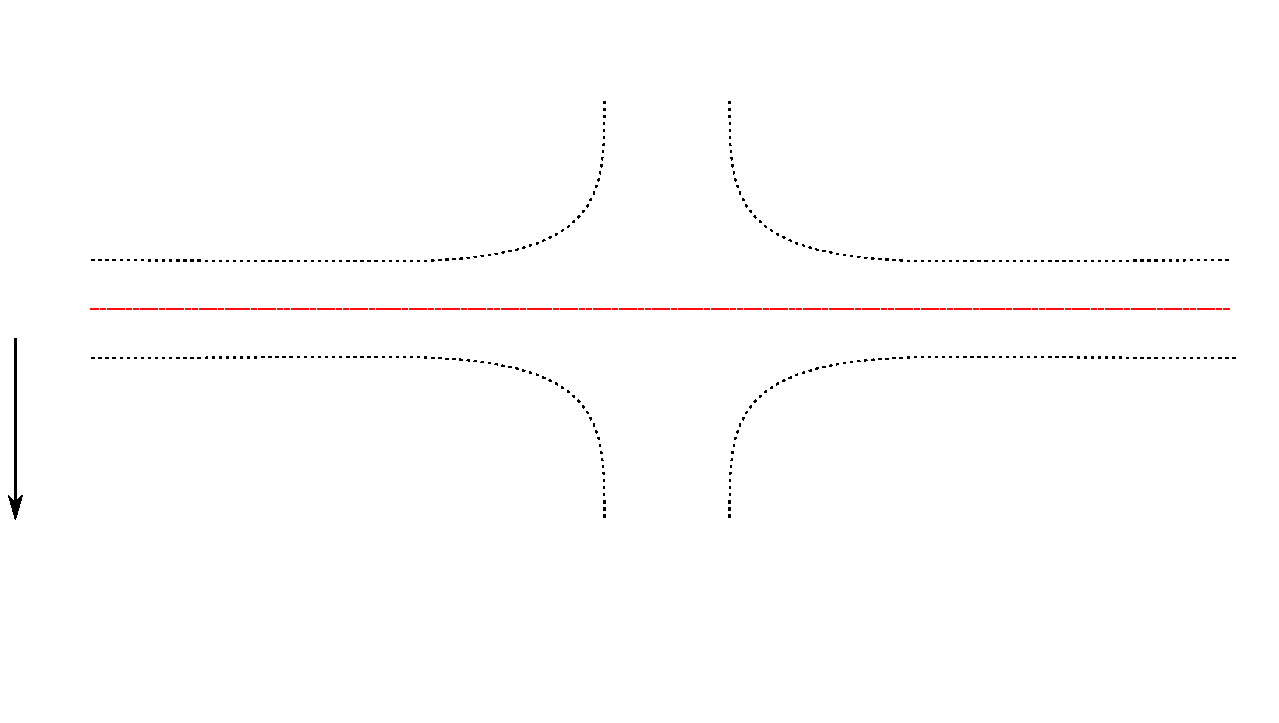
\includegraphics[width=\unitlength,page=1]{../plots/CounterDiffusionFlame_sketch_rotated2.pdf}}\put(0.50187804,0.002595){\color[rgb]{0,0,0}\makebox(0,0)[lt]{\lineheight{1.25}\smash{\begin{tabular}[t]{l}$6\hat{L}$\end{tabular}}}}\put(0,0){\includegraphics[width=\unitlength,page=2]{../plots/CounterDiffusionFlame_sketch_rotated2.pdf}}\put(0.73588839,0.30040165){\color[rgb]{0,0,0}\makebox(0,0)[lt]{\lineheight{1.25}\smash{\begin{tabular}[t]{l}\text{Stagnation plane}\\\end{tabular}}}}\put(0,0){\includegraphics[width=\unitlength,page=3]{../plots/CounterDiffusionFlame_sketch_rotated2.pdf}}\put(0.28154156,0.39441284){\color[rgb]{0,0,0}\makebox(0,0)[t]{\lineheight{1.25}\smash{\begin{tabular}[t]{c}\text{Adiabatic wall}\end{tabular}}}}\put(0.77020774,0.39621194){\color[rgb]{0,0,0}\makebox(0,0)[t]{\lineheight{1.25}\smash{\begin{tabular}[t]{c}\text{Adiabatic wall}\end{tabular}}}}\put(0.77020774,0.04390421){\color[rgb]{0,0,0}\makebox(0,0)[t]{\lineheight{1.25}\smash{\begin{tabular}[t]{c}\text{Adiabatic wall}\end{tabular}}}}\put(0.28264939,0.04291605){\color[rgb]{0,0,0}\makebox(0,0)[t]{\lineheight{1.25}\smash{\begin{tabular}[t]{c}\text{Adiabatic wall}\end{tabular}}}}\put(0.23597805,0.28618457){\color[rgb]{0,0,0}\makebox(0,0)[lt]{\lineheight{1.25}\smash{\begin{tabular}[t]{l}\text{Flame}\\\end{tabular}}}}\put(0,0){\includegraphics[width=\unitlength,page=4]{../plots/CounterDiffusionFlame_sketch_rotated2.pdf}}\put(0.06924897,0.13479347){\color[rgb]{0,0,0}\rotatebox{90}{\makebox(0,0)[lt]{\lineheight{1.25}\smash{\begin{tabular}[t]{l}\text{Pressure outlet}\end{tabular}}}}}\put(0.99712048,0.14305974){\color[rgb]{0,0,0}\rotatebox{90}{\makebox(0,0)[lt]{\lineheight{1.25}\smash{\begin{tabular}[t]{l}\text{Pressure outlet}\end{tabular}}}}}\put(0,0){\includegraphics[width=\unitlength,page=5]{../plots/CounterDiffusionFlame_sketch_rotated2.pdf}}\end{picture}\endgroup \caption{Schematic representation of the counterflow configuration.}
	\label{fig:CDFScheme}
\end{figure*}
The counterflow diffusion flame is a canonical configuration used to study the structure of non-premixed flames. In its most basic configuration it consists of two oppositely situated jets. The fuel (possibly mixed with some inert component such as nitrogen) is fed into the system by one of the jets, while the other jet feeds air to the system, thereby establishing a stagnation point flow. Upon contact, the reactants produce a flame which is located in the vicinity of the stagnation plane. A diagram of the setup can be seen in \cref{fig:CDFScheme}. This simple configuration has been subject of study for decades  because it provides a simple way of creating a strained diffusion flame, which proves to be useful when studying the flame structure, extinction limits or production of pollutants of flames \cite{pandyaStructureFlatCounterFlow1964} \cite{spaldingTheoryMixingChemical1961} \cite{keyesFlameSheetStarting1987}. By assuming an infinite injector diameter and self-similarity of the solution, it is possible to reduce the governing equations to a one-dimensional formulation (see e.g. the textbook of Kee \cite{keeChemicallyReactingFlow2003}). As a means of validating our implementation we compare the results with the solution of the one-dimensional self-similar problem calculated with \lstinline|BVP4|, a fourth order finite difference boundary value problem solver provided by \lstinline|MATLAB|. 

The combustion of a methane-nitrogen mixture with air was simulated using the \BoSSS code. The mass composition of the fuel inlet was assumed to be  $Y^0_{\ch{CH4}} = 0.2$ and $Y^0_{\ch{N2}} = 0.8$, and the oxidizer inlet corresponds to air with   $Y^0_{\ch{O2}} = 0.23$ and $Y^0_{\ch{N2}} = 0.77$. Because we are dealing with an open system, the thermodynamic pressure $\hat p_0$ is constant and set to the ambient pressure of $\SI{101325}{\pascal}$. As noted by Sung et al., \cite{sungStructuralResponseCounterflow1995} although the form of the inlet velocity profiles does have an influence on the solution of the problem, its effect on the solution near the flame zone is rather small. Nevertheless, as mentioned before the solution of the self-similar one-dimensional problem assumed an infinite injector diameter, which implies that the upstream velocity field has to be constant. Based on this fact we set the velocity profile of both inlets as a plug flow. Following combinations of inlet velocities were calculated:
\begin{itemize}
	\item  Low inlet velocities:  $u^0_{\text{fuel}} = \SI{0.048}{\meter \per \second}$ and  $u^0_{\text{oxidizer}} = \SI{0.144}{\meter \per \second}$,
	\item Medium inlet velocities:  $u^0_{\text{fuel}} = \SI{0.12}{\meter \per \second}$ and  $u^0_{\text{oxidizer}} = \SI{0.36}{\meter \per \second}$
	\item High inlet velocities: $u^0_{\text{fuel}}  = \SI{0.24}{\meter \per \second}$ and   $u^0_{\text{oxidizer}} = \SI{0.72}{\meter \per \second}$
\end{itemize}
By using as definition of the strain rate the maximum axial velocity gradient, the calculated strains for the three cases mentioned above are $\SI{34}{\per\second}$, $\SI{76}{\per\second}$ and $\SI{155}{\per\second}$, respectively. The temperature of both inlets is \SI{300}{\kelvin}. The separation between both jets $\hat L$ is equal to $\SI{0.02}{\meter}$, and the length of the inlet opening $\hat D$ is $\SI{0.02}{\meter}$. The left and right domain boundaries are selected to be at a distance $3\hat L$ of the center. A non-unity but constant Lewis number formulation is used,with  
$\Lewis_{\ch{CH4}} =  0.97 $ , $\Lewis_{\ch{O2}} = 1.11 $, $\Lewis_{\ch{H2O}} = 0.83 $ and $\Lewis_{\ch{CO2}} = 1.39 $.\cite{smookePremixedNonpremixedTest1991} The heat capacity of each component is evaluated locally from NASA polynomials, and the mixture heat capacity is calculated with \cref{eq:nondim_cpmixture}.
\tikzset{external/export next=false}
\begin{figure}[t!]
	\centering
	\pgfplotsset{
		compat=1.3,
		tick align = outside,
		yticklabel style={/pgf/number format/fixed}, 
	}
	\begin{tikzpicture}	
	\begin{axis}[
	set layers=standard,
	width=0.75\linewidth,
	height=6cm,
	ymode = log,
	xlabel=Iteration number,
	xmin = 0,
	ylabel=Residual and trust region $\delta$,
	xtick = {0,2,...,32},
	ytickten = {-16,-12,...,12},
	ymax = 1e9,
	legend style = {at = {(0.1,0.1)}, anchor = south west},
	]
	\addplot[ orange, mark =o, mark size = 2.5pt] file{data/ConvergenceStory_CounterDiffusionFlame/residuals3.txt};\addlegendentry{$	\| \mathcal{A}(\myvector{U}_{n}) \|_2 $};	
	\addplot[ blue, mark =square*, mark size = 2pt] file{data/ConvergenceStory_CounterDiffusionFlame/delta3.txt}; \addlegendentry{$\delta$};	
	\node[draw, ] at (80,16.3) {Flame sheet calculation};
	\draw [dashed,thick] (180, \pgfkeysvalueof{/pgfplots/ymin}) -- (180, \pgfkeysvalueof{/pgfplots/ymax});
	\node[draw, ] at (240,16.3) {Finite rate chemistry calculation};
	\end{axis} 
	\end{tikzpicture}
	\caption{Convergence history of the diffusion flame in the counterflow configuration, with a maximum strain value of $165.1 $\si{s^{-1}}}
	\label{fig:CDF_ConvergenceStory}
\end{figure} 

In \cref{fig:CDF_ConvergenceStory} the convergence history obtained for a typical calculation of the counter diffusion flame is presented. The solution of the flame sheet calculation requires 17 iterations until convergence is reached. The obtained solution is used as a starting value for the finite chemical rate calculation, which only needs 10 iterations until convergence is reached. We note that because the flame sheet calculation is only used as an approximation of the final solution, a low polynomial degree can be used. For the flame sheet calculation $k = 2$ was chosen, resulting in a rather small system with 26,880 degrees of freedom. For the finite rate calculation $k = 4$ was used, which resulted in a system with 174,110 degrees of freedom.  With the above-mentioned another advantage of the approach of using the flame sheet calculation for two-dimensional simulations can be highlighted. The initial estimate can be found relatively easily for a system with few degrees of freedom. Using the solution found as the initial estimate has the consequence that Newton's algorithm for the complete problem (which has many more degrees of freedom) only needs a few iterations to find a solution. 

Because we are solving a two-dimensional configuration, in order to be able to compare our results with the ones obtained from the one-dimensional representation, the temperature, mass fractions and velocity profiles are extracted along the centerline of the system shown as the dashed line in \cref{fig:CDFScheme}. In \cref{fig:BoSSS_1D_Comparison_velocity} a comparison of the axial velocities calculated with \BoSSS and the one-dimensional solution is shown. While for the high strain case the results agree closely, for lower strains a discrepancy is observed. Recall that the derivation of the one-dimensional approximation assumes a constant velocity field incoming to the flame zone in order to obtain a self-similar solution. In the case of the two-dimensional configuration presented here, the border effects do have an influence on the centerline, which disrupts the self-similarity. This effect is more pronounced for low velocities, which explains the discrepancy between curves. Similarly, In \cref{fig:BoSSS_1D_Comparison} the temperature and mass fraction fields are presented. Again, a discrepancy is observed for low strains, but results show a good agreement for higher inlet velocities. It can also be observed how, as expected, \cite{fernandez-tarrazoSimpleOnestepChemistry2006} at higher strains a significant penetration (leakage) of oxygen across the flame is present. Finally, in \cref{fig:TempAndReacFields} the two-dimensional temperature, velocity and reaction rate fields for the case (a) are shown. 
We note that the solution of this configuration showed singularities in the boundary points where the inlet and wall meet. This fact made hard to realize an $h$-convergence study for the complete domain. Based on this we decided to analyze a flame configuration that does not exhibit this behaviour, as shown in the next section.

\begin{figure}[t!]
	\pgfplotsset{
		group/xticklabels at=edge bottom,
		legend style = {
			at ={ (0.5,1), anchor= north east}
		},
		unit code/.code={\si{#1}}
	}
	\centering
	\begin{tikzpicture}
	\begin{groupplot}[
	group style={
		group name=my plots,
		group size=3 by 1,
		x descriptions at=edge bottom,
		ylabels at = edge left,
	},
	width= 0.21\textwidth ,
	height= 0.21\textwidth ,
	xlabel = $x$,
	x unit=\meter,
	y unit = \meter \per \second,
	ylabel= Axial-velocity,
	change x base=true,
	x SI prefix=centi,	
	change y base = true,
	y SI prefix=centi,
	max space between ticks=1000pt,
	try min ticks=5,
	]
	\nextgroupplot[title = {\textbf{Case (a)}}]
	\addplot+[color=black, no marks, thick] table {data/DataStrainSweep/2/FullVelocityX_BOSSS.txt}; \addlegendentry{\BoSSS}
	\addplot+[color=black, no marks, dashed]table {data/DataStrainSweep/2/FullVelocityX_MATLAB2.txt};\addlegendentry{1D}
	\nextgroupplot[title = {\textbf{Case (b)}}]
	\addplot+[color=black, no marks, thick] table {data/DataStrainSweep/5/FullVelocityX_BOSSS.txt};\addlegendentry{\BoSSS}
	\addplot+[color=black, no marks, dashed]table {data/DataStrainSweep/5/FullVelocityX_MATLAB.txt};\addlegendentry{1D}
	\nextgroupplot [title = {\textbf{Case (c)}}]
	\addplot+[color=black, no marks, thick] table {data/DataStrainSweep/11/FullVelocityX_BOSSS.txt};\addlegendentry{\BoSSS}
	\addplot+[color=black, no marks, dashed]table {data/DataStrainSweep/11/FullVelocityX_MATLAB.txt};\addlegendentry{1D}
	\end{groupplot}
	\end{tikzpicture}
	\caption{ Comparison of the axial velocity calculated with \BoSSS and the one-dimensional approximation. }
	\label{fig:BoSSS_1D_Comparison_velocity}
\end{figure}
\tikzexternaldisable
%\tikzset{external/export next=false}%%%%%%%%%%%%%%%%%%%%%%%%%%%%%%%%%%%%%%%%%%%%%%%%%%%%%%%%%%%%%%%%%%%%%%%%%%%%%%%%%%%%%%%%%%%%%%%%%%%%%%%
\begin{figure}[b!]
	\centering
	\pgfplotsset{
		width=0.65\textwidth,
		height = 0.2\textwidth,
		compat=1.3,
		tick align = outside,
		yticklabel style={/pgf/number format/fixed}, 
	}
	\begin{tikzpicture}[baseline]
	\begin{axis}[
	title = {\textbf{Case (a)}},
	ylabel= Temperature ,
	axis y line*=left,
	ymin = 300,
	y unit= K, 
	change x base=true,
	x SI prefix=centi,
	xtick=\empty,
	xticklabel=\empty,
	]
	\addplot+[color=cyan, no marks, thick] table {data/DataStrainSweep/2/FullTemperature_BOSSS.txt};
	\addplot+[color=cyan, no marks, dashed]table {data/DataStrainSweep/2/FullTemperature_MATLAB.txt};
	\end{axis}
	
	\begin{axis}[
	x tick label style={
		/pgf/number format/.cd,
		precision=3,
		/tikz/.cd
	},
	ymin=0.0, ymax =0.25, 
	ylabel= Mass fraction,
	legend style={at={(0.8,0.7)}, anchor=north east},
	axis y line*=right,
	change x base=true,
	x SI prefix=centi,
	xtick=\empty,
	xticklabel=\empty,
	] 	
	\addplot+[color=black, no marks, thick,solid] table {data/DataStrainSweep/2/FullMassFraction0_BOSSS.txt};
	\addplot+[color=blue,no marks,thick,solid] table {data/DataStrainSweep/2/FullMassFraction1_BOSSS.txt};
	\addplot+[color=green, no marks,thick,solid] table {data/DataStrainSweep/2/FullMassFraction2_BOSSS.txt};
	\addplot+[color=red, no marks,thick,solid] table {data/DataStrainSweep/2/FullMassFraction3_BOSSS.txt};
	\addplot+[color=black,no marks, dashed] table {data/DataStrainSweep/2/FullMassFraction0_Matlab.txt};
	\addplot+[color=blue,no marks, dashed] table {data/DataStrainSweep/2/FullMassFraction1_Matlab.txt};
	\addplot+[color=green,no marks, dashed] table {data/DataStrainSweep/2/FullMassFraction2_Matlab.txt};
	\addplot+[color=red,no marks, dashed] table {data/DataStrainSweep/2/FullMassFraction3_Matlab.txt};	
	\end{axis}
	\end{tikzpicture}	
	\begin{tikzpicture}[baseline]
	\begin{axis}[
	title = {\textbf{Case (b)}},
	ylabel= Temperature ,
	axis y line*=left,
	ymin = 300,
	y unit= K, 
	change x base=true,
	x SI prefix=centi,
	xtick=\empty,
	xticklabel=\empty,
	]
	\addplot+[color=cyan, no marks, thick] table {data/DataStrainSweep/5/FullTemperature_BOSSS.txt};
	\addplot+[color=cyan, no marks, dashed]table {data/DataStrainSweep/5/FullTemperature_MATLAB.txt};
	\end{axis} 	
	\begin{axis}[
	x tick label style={
		/pgf/number format/.cd,
		precision=3,
		/tikz/.cd
	},
	ymin=0.0, ymax =0.25, 
	ylabel= Mass fraction,
	axis y line*=right,
	change x base=true,
	x SI prefix=centi,
	xtick=\empty,
	xticklabel=\empty,
	] 	
	\addplot+[color=black, no marks, thick,solid] table {data/DataStrainSweep/5/FullMassFraction0_BOSSS.txt};
	\addplot+[color=blue,no marks,thick,solid] table {data/DataStrainSweep/5/FullMassFraction1_BOSSS.txt};
	\addplot+[color=green, no marks,thick,solid] table {data/DataStrainSweep/5/FullMassFraction2_BOSSS.txt};
	\addplot+[color=red, no marks,thick,solid] table {data/DataStrainSweep/5/FullMassFraction3_BOSSS.txt};
	\addplot+[color=black,no marks, dashed] table {data/DataStrainSweep/5/FullMassFraction0_Matlab.txt};
	\addplot+[color=blue,no marks, dashed] table {data/DataStrainSweep/5/FullMassFraction1_Matlab.txt};
	\addplot+[color=green,no marks, dashed] table {data/DataStrainSweep/5/FullMassFraction2_Matlab.txt};
	\addplot+[color=red,no marks, dashed] table {data/DataStrainSweep/5/FullMassFraction3_Matlab.txt};	
	\end{axis}
	\end{tikzpicture}	 	
	\begin{tikzpicture}[baseline]
	\begin{axis}[
	title = {\textbf{Case (c)}},
	xlabel=$x$,
	ylabel= Temperature ,
	axis y line*=left,
	ymin = 300,
	x unit=m,
	y unit= K, 
	change x base=true,
	x SI prefix=centi
	]
	\addplot[color=cyan, no marks, thick] table {data/DataStrainSweep/11/FullTemperature_BOSSS.txt}; \label{TemperatureBosss}
	\addplot[color=cyan, no marks, dashed]table {data/DataStrainSweep/11/FullTemperature_MATLAB.txt}; \label{TemperatureMatlab}
	\end{axis} 	
	\begin{axis}[
	x tick label style={
		/pgf/number format/.cd,
		precision=3,
		/tikz/.cd
	},
	ymin=0.0, ymax =0.25, 
	xlabel=$x$,
	ylabel= Mass fraction,
	x unit=m,
	axis y line*=right,
	change x base=true,
	x SI prefix=centi
	]
	\addplot[color=black, no marks, thick,solid] table {data/DataStrainSweep/11/FullMassFraction0_BOSSS.txt}; \label{MF0_BOSSS}
	\addplot[color=blue,no marks,thick,solid] table {data/DataStrainSweep/11/FullMassFraction1_BOSSS.txt}; 	\label{MF1_BOSSS}
	\addplot[color=green, no marks,thick,solid] table {data/DataStrainSweep/11/FullMassFraction2_BOSSS.txt}; 	\label{MF2_BOSSS}
	\addplot[color=red, no marks,thick,solid] table {data/DataStrainSweep/11/FullMassFraction3_BOSSS.txt}; 	\label{MF3_BOSSS}
	\addplot[color=black,no marks, dashed] table {data/DataStrainSweep/11/FullMassFraction0_Matlab.txt};\label{MF0_MATLAB}
	\addplot[color=blue,no marks, dashed] table {data/DataStrainSweep/11/FullMassFraction1_Matlab.txt};\label{MF1_MATLAB}	
	\addplot[color=green,no marks, dashed] table {data/DataStrainSweep/11/FullMassFraction2_Matlab.txt};\label{MF2_MATLAB}	
	\addplot[color=red,no marks, dashed] table {data/DataStrainSweep/11/FullMassFraction3_Matlab.txt};\label{MF3_MATLAB}	
	\end{axis}
	\node[draw,anchor=south east] at (11.0cm,0.4cm) {
		\begin{tabular}{ccl}
		$T$:& \BoSSS \ref{TemperatureBosss} ;& 1D \tikz{\ref{TemperatureMatlab}}  \\
		$Y_{\ch{CH4}}$:& \BoSSS \tikz{\ref{MF0_BOSSS}} ;& 1D \tikz{\ref{MF0_MATLAB}} \\
		$Y_{\ch{O2}}$:& \BoSSS \tikz{\ref{MF1_BOSSS}} ;& 1D \tikz{\ref{MF1_MATLAB}} \\
		$Y_{\ch{CO2}}$:& \BoSSS \tikz{\ref{MF2_BOSSS}} ;& 1D \tikz{\ref{MF2_MATLAB}}  \\
		$Y_{\ch{H2O}}$:& \BoSSS \tikz{\ref{MF3_BOSSS}} ;& 1D \tikz{\ref{MF3_MATLAB}}  
		\end{tabular}
	};
	\end{tikzpicture}	
	\caption{ Comparison of temperature and mass fraction fields obtained with \BoSSS and the one-dimensional approximation.}
	\label{fig:BoSSS_1D_Comparison}
\end{figure}
\begin{figure}[tb!]
	\centering
	\def\svgwidth{0.8\textwidth}
	\begingroup \makeatletter \providecommand\color[2][]{\errmessage{(Inkscape) Color is used for the text in Inkscape, but the package 'color.sty' is not loaded}\renewcommand\color[2][]{}}\providecommand\transparent[1]{\errmessage{(Inkscape) Transparency is used (non-zero) for the text in Inkscape, but the package 'transparent.sty' is not loaded}\renewcommand\transparent[1]{}}\providecommand\rotatebox[2]{#2}\newcommand*\fsize{\dimexpr\f@size pt\relax}\newcommand*\lineheight[1]{\fontsize{\fsize}{#1\fsize}\selectfont}\ifx\svgwidth\undefined \setlength{\unitlength}{578.08882105bp}\ifx\svgscale\undefined \relax \else \setlength{\unitlength}{\unitlength * \real{\svgscale}}\fi \else \setlength{\unitlength}{\svgwidth}\fi \global\let\svgwidth\undefined \global\let\svgscale\undefined \makeatother \begin{picture}(1,0.56429776)\lineheight{1}\setlength\tabcolsep{0pt}\put(0,0){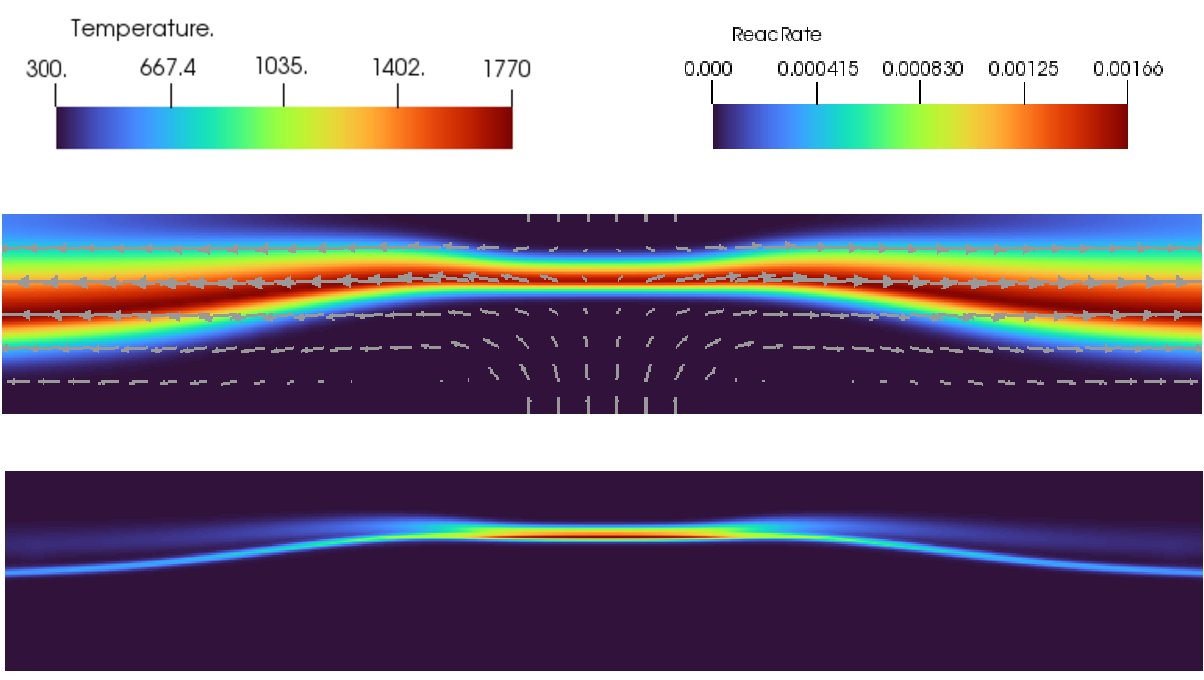
\includegraphics[width=\unitlength,page=1]{../plots/CDF_Results.pdf}}\end{picture}\endgroup \caption{Calculated temperature and velocity fields (top picture) and reaction rate (second picture) of the counter diffusion flame configuration, case (a). The unit of the temperature is \si{K} and of the reaction rate \si{\kilo\mole \per \meter \cubed \per \second}. }
	\label{fig:TempAndReacFields}
\end{figure}
\tikzexternalenable

\subsection{Chambered diffusion flame}\label{ss:UDF}


\begin{figure}[b!]
	\begin{center}
		\def\svgwidth{0.35\textwidth}
		\begingroup \makeatletter \providecommand\color[2][]{\errmessage{(Inkscape) Color is used for the text in Inkscape, but the package 'color.sty' is not loaded}\renewcommand\color[2][]{}}\providecommand\transparent[1]{\errmessage{(Inkscape) Transparency is used (non-zero) for the text in Inkscape, but the package 'transparent.sty' is not loaded}\renewcommand\transparent[1]{}}\providecommand\rotatebox[2]{#2}\newcommand*\fsize{\dimexpr\f@size pt\relax}\newcommand*\lineheight[1]{\fontsize{\fsize}{#1\fsize}\selectfont}\ifx\svgwidth\undefined \setlength{\unitlength}{943.88190322bp}\ifx\svgscale\undefined \relax \else \setlength{\unitlength}{\unitlength * \real{\svgscale}}\fi \else \setlength{\unitlength}{\svgwidth}\fi \global\let\svgwidth\undefined \global\let\svgscale\undefined \makeatother \begin{picture}(1,0.84935754)\lineheight{1}\setlength\tabcolsep{0pt}\put(0,0){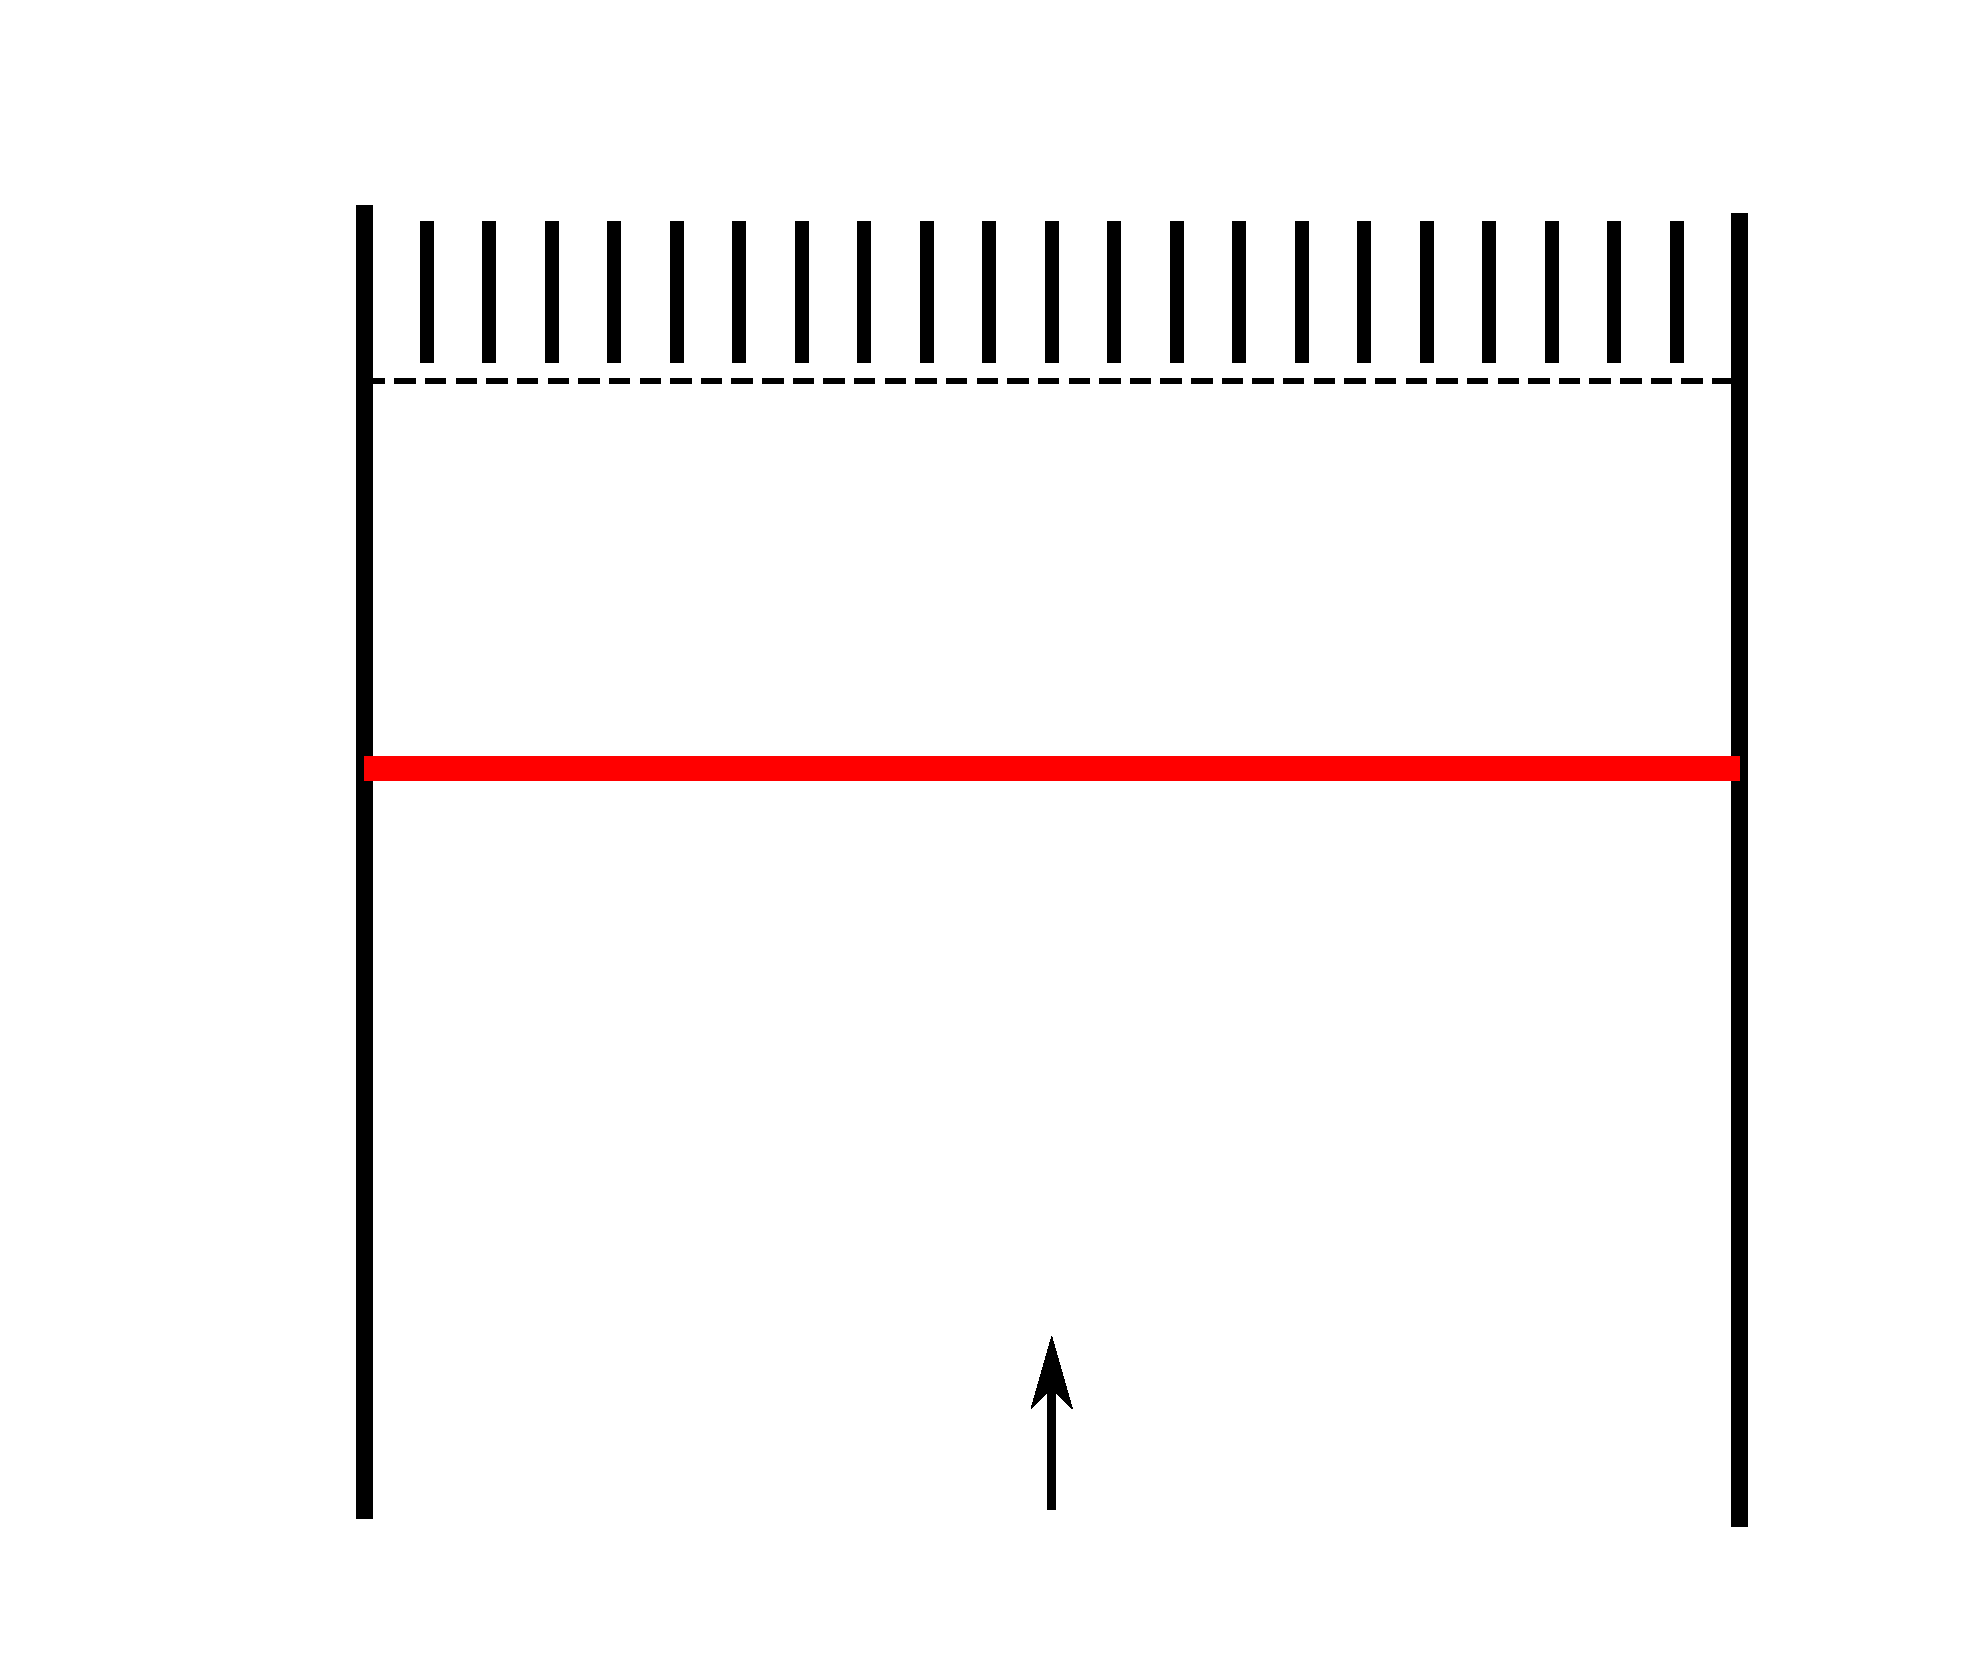
\includegraphics[width=\unitlength,page=1]{../plots/UnstrainedFlameConfig.pdf}}\put(0.50835425,0.17720939){\color[rgb]{0,0,0}\makebox(0,0)[lt]{\lineheight{1.25}\smash{\begin{tabular}[t]{l}Fuel\end{tabular}}}}\put(0,0){\includegraphics[width=\unitlength,page=2]{../plots/UnstrainedFlameConfig.pdf}}\put(0.48865082,0.47743759){\color[rgb]{0,0,0}\makebox(0,0)[lt]{\lineheight{1.25}\smash{\begin{tabular}[t]{l}Flame\end{tabular}}}}\put(0.67802482,0.8252095){\color[rgb]{0,0,0}\makebox(0,0)[lt]{\lineheight{1.25}\smash{\begin{tabular}[t]{l}Products\end{tabular}}}}\put(0.37592055,0.8252095){\color[rgb]{0,0,0}\makebox(0,0)[lt]{\lineheight{1.25}\smash{\begin{tabular}[t]{l}Oxidizer\end{tabular}}}}\put(0.15496603,0.19893189){\color[rgb]{0,0,0}\rotatebox{90}{\makebox(0,0)[lt]{\lineheight{1.25}\smash{\begin{tabular}[t]{l}Periodic boundary\end{tabular}}}}}\put(0.9420434,0.18958958){\color[rgb]{0,0,0}\rotatebox{90}{\makebox(0,0)[lt]{\lineheight{1.25}\smash{\begin{tabular}[t]{l}Periodic boundary\end{tabular}}}}}\put(0.40312388,0.00958245){\color[rgb]{0,0,0}\makebox(0,0)[lt]{\lineheight{1.25}\smash{\begin{tabular}[t]{l}Velocity inlet\end{tabular}}}}\put(0.38405371,0.60552565){\color[rgb]{0,0,0}\makebox(0,0)[lt]{\lineheight{1.25}\smash{\begin{tabular}[t]{l}Pressure outlet\end{tabular}}}}\put(0.90275774,0.64694849){\color[rgb]{0,0,0}\makebox(0,0)[lt]{\lineheight{1.25}\smash{\begin{tabular}[t]{l}x = 0\end{tabular}}}}\put(0,0){\includegraphics[width=\unitlength,page=3]{../plots/UnstrainedFlameConfig.pdf}}\put(0.06707395,0.67423724){\color[rgb]{0,0,0}\makebox(0,0)[lt]{\lineheight{1.25}\smash{\begin{tabular}[t]{l}y\end{tabular}}}}\put(0.0313179,0.55432415){\color[rgb]{0,0,0}\makebox(0,0)[lt]{\lineheight{1.25}\smash{\begin{tabular}[t]{l}x\end{tabular}}}}\put(0,0){\includegraphics[width=\unitlength,page=4]{../plots/UnstrainedFlameConfig.pdf}}\end{picture}\endgroup \vspace{0.2cm}
		\caption{Schematic representation of the chambered diffusion flame configuration. }
		\label{fig:chamberedDifFlame}
	\end{center}	
\end{figure}
The chambered diffusion flame configuration has served as a model for many theoretical studies related to diffusion flames\cite{matalonEffectThermalExpansion2010,rameauNumericalBifurcationChambered1985,matalonDiffusionFlamesChamber1980} A scheme of the configuration can be seen in \cref{fig:chamberedDifFlame}. Fuel is injected at a constant rate into the bottom of a small insulated chamber, while oxidant diffuses into the system against the direction of flow. Constant conditions at the outlet of the chamber are achieved by a rapid renewal of the flow of oxidant.  Under these conditions a planar flame forms far away from the walls, which allows a one-dimensional description of the flame structure.
The fuel inlet into the chamber is modelled with a velocity inlet boundary condition \cref{eq:bc_d}, while the flow outlet at the top is considered an outlet as given by \cref{eq:bc_OD}. Since we are interested in the flame in wall distance, it is sufficient to set the remaining boundary conditions as periodic boundaries. This effectively transforms the problem into a pseudo two-dimensional configuration. 


\begin{figure}[t!]
	\centering
	\pgfplotsset{width=0.34\textwidth, compat=1.3}
	\begin{tikzpicture}
	\begin{groupplot}[
	group style={
		group name= group,
		group size=2 by 2,
		ylabels at=edge left,
		horizontal sep = 2.5cm,
		vertical sep = 1.5cm,
	},
	xtick={2^-8,2^-7,2^-6, 2^-5},
	xticklabels = {$2^{-8}$,$2^{-7}$,$2^{-6}$,$2^{-5}$},
	xlabel=Cell length $h$,
	xmajorgrids,
	ymajorgrids,
	legend style={at={(1,0)}, anchor=south east},
	]
	\nextgroupplot[xmode=log, ymode=log,ylabel = $\LtwoNorm{ u_x - u_{x,\text{fine}}}$,]
	\addplot+[color=black, dashed] table {data/UnstrainedDiffFlame_ConvStudy/WithCombustion/VelocityXDG1Data.txt};
	\addlegendentry{$k=1$};
	\addplot[solid,  forget plot] table [   
	x=x,
	y={create col/linear regression={y=y,
			variance list={10000,800,600,500,400,200,100}}}]
	{data/UnstrainedDiffFlame_ConvStudy/WithCombustion/VelocityXDG1Data.txt}
	coordinate [pos=0.75] (A)
	coordinate [pos=0.90] (B)
	;
	\xdef\slopeXA{\pgfplotstableregressiona}			
	\draw (A) |- (B)
	node [pos=0.55,anchor= west]
	{\pgfmathprintnumber{\slopeXA}};			
	\addplot+[color=black, dashed] table {data/UnstrainedDiffFlame_ConvStudy/WithCombustion/VelocityXDG2Data.txt};
	\addlegendentry{$k=2$};
	\addplot[solid, forget plot] table [   
	x=x,
	y={create col/linear regression={y=y,
			variance list={10000,800,600,500,400,200,100}				
	}}]
	{data/UnstrainedDiffFlame_ConvStudy/WithCombustion/VelocityXDG2Data.txt}
	coordinate [pos=0.75] (A)
	coordinate [pos=0.90] (B)
	;
	\xdef\slopeXB{\pgfplotstableregressiona}			
	\draw (A) |- (B)
	node [pos=0.55,anchor=  west]
	{\pgfmathprintnumber{\slopeXB}};			
	\addplot+[color=black, dashed] table {data/UnstrainedDiffFlame_ConvStudy/WithCombustion/VelocityXDG3Data.txt};
	\addlegendentry{$k=3$};			
	\addplot[solid, forget plot] table [   
	x=x,
	y={create col/linear regression={y=y,
			variance list={10000,800,600,500,400,200,100}}}]
	{data/UnstrainedDiffFlame_ConvStudy/WithCombustion/VelocityXDG3Data.txt}
	coordinate [pos=0.75] (A)
	coordinate [pos=0.90] (B)
	;
	\xdef\slopeXC{\pgfplotstableregressiona}			
	\draw (A) |- (B)
	node [pos=0.55,anchor=south west]
	{\pgfmathprintnumber{\slopeXC}};			
	\addplot+[color=black, dashed] table {data/UnstrainedDiffFlame_ConvStudy/WithCombustion/VelocityXDG4Data.txt};
	\addlegendentry{$k=4$};
	\addplot[solid, forget plot] table [   
	x=x,
	y={create col/linear regression={y=y,
			variance list={10000,800,600,500,400,200,100}}}]
	{data/UnstrainedDiffFlame_ConvStudy/WithCombustion/VelocityXDG4Data.txt}
	coordinate [pos=0.75] (A)
	coordinate [pos=0.9] (B)
	;
	\xdef\slopeXD{\pgfplotstableregressiona}			
	\draw (A) |- (B)
	node [pos=0.55,anchor=south west]
	{\pgfmathprintnumber{\slopeXD}};				
	\nextgroupplot[xmode=log, ymode=log,	ylabel = $ \LtwoNorm{T - T_{\text{fine}}}$,]
	\addplot+[color=black, dashed] table {data/UnstrainedDiffFlame_ConvStudy/WithCombustion/TemperatureDG1Data.txt};
	\addlegendentry{$k=1$};
	\addplot[solid,  forget plot] table [   
	x=x,
	y={create col/linear regression={y=y,
			variance list={10000,800,600,500,400,200,100}}}]
	{data/UnstrainedDiffFlame_ConvStudy/WithCombustion/TemperatureDG1Data.txt}
	coordinate [pos=0.75] (A)
	coordinate [pos=0.90] (B)
	;
	\xdef\slopeXA{\pgfplotstableregressiona}			
	\draw (A) |- (B)
	node [pos=0.55,anchor= west]
	{\pgfmathprintnumber{\slopeXA}};			
	\addplot+[color=black, dashed] table {data/UnstrainedDiffFlame_ConvStudy/WithCombustion/TemperatureDG2Data.txt};
	\addlegendentry{$k=2$};
	\addplot[solid, forget plot] table [   
	x=x,
	y={create col/linear regression={y=y,
			variance list={10000,800,600,500,400,200,100}}}]
	{data/UnstrainedDiffFlame_ConvStudy/WithCombustion/TemperatureDG2Data.txt}
	coordinate [pos=0.75] (A)
	coordinate [pos=0.85] (B)
	;
	\xdef\slopeXB{\pgfplotstableregressiona}			
	\draw (A) |- (B)
	node [pos=0.55,anchor=  west]
	{\pgfmathprintnumber{\slopeXB}};			
	\addplot+[color=black, dashed] table {data/UnstrainedDiffFlame_ConvStudy/WithCombustion/TemperatureDG3Data.txt};
	\addlegendentry{$k=3$};			
	\addplot[solid, forget plot] table [   
	x=x,
	y={create col/linear regression={y=y,
			variance list={10000,800,600,500,400,200,100}}}]
	{data/UnstrainedDiffFlame_ConvStudy/WithCombustion/TemperatureDG3Data.txt}
	coordinate [pos=0.75] (A)
	coordinate [pos=0.90] (B)
	;
	\xdef\slopeXC{\pgfplotstableregressiona}			
	\draw (A) |- (B)
	node [pos=0.55,anchor=south west]
	{\pgfmathprintnumber{\slopeXC}};			
	\addplot+[color=black, dashed] table {data/UnstrainedDiffFlame_ConvStudy/WithCombustion/TemperatureDG4Data.txt};
	\addlegendentry{$k=4$};
	\addplot[solid, forget plot] table [   
	x=x,
	y={create col/linear regression={y=y,
			variance list={100000,800000,600,500,400,200,100}}}]
	{data/UnstrainedDiffFlame_ConvStudy/WithCombustion/TemperatureDG4Data.txt}
	coordinate [pos=0.75] (A)
	coordinate [pos=0.9] (B)
	;
	\xdef\slopeXD{\pgfplotstableregressiona}			
	\draw (A) |- (B)
	node [pos=0.55,anchor=south west]
	{\pgfmathprintnumber{\slopeXD}};	
	\nextgroupplot[ xmode=log, ymode=log,	ylabel=$\LtwoNorm{ Y_{\ch{CH4}} - Y_{{\ch{CH4}},\text{fine}} }$,]
	\addplot+[color=black, dashed] table {data/UnstrainedDiffFlame_ConvStudy/WithCombustion/MassFraction0DG1Data.txt};
	\addlegendentry{$k=1$};
	\addplot[solid,  forget plot] table [   
	x=x,
	y={create col/linear regression={y=y,
			variance list={10000,800,600,500,400,200,100}}}]
	{data/UnstrainedDiffFlame_ConvStudy/WithCombustion/MassFraction0DG1Data.txt}
	coordinate [pos=0.75] (A)
	coordinate [pos=0.90] (B)
	;
	\xdef\slopeXA{\pgfplotstableregressiona}			
	\draw (A) |- (B)
	node [pos=0.55,anchor= west]
	{\pgfmathprintnumber{\slopeXA}};			
	\addplot+[color=black, dashed] table {data/UnstrainedDiffFlame_ConvStudy/WithCombustion/MassFraction0DG2Data.txt};
	\addlegendentry{$k=2$};
	\addplot[solid, forget plot] table [   
	x=x,
	y={create col/linear regression={y=y,
			variance list={10000,800,600,500,400,200,100}}}]
	{data/UnstrainedDiffFlame_ConvStudy/WithCombustion/MassFraction0DG2Data.txt}
	coordinate [pos=0.75] (A)
	coordinate [pos=0.90] (B)
	;
	\xdef\slopeXB{\pgfplotstableregressiona}			
	\draw (A) |- (B)
	node [pos=0.55,anchor=  west]
	{\pgfmathprintnumber{\slopeXB}};			
	\addplot+[color=black, dashed] table {data/UnstrainedDiffFlame_ConvStudy/WithCombustion/MassFraction0DG3Data.txt};
	\addlegendentry{$k=3$};			
	\addplot[solid, forget plot] table [   
	x=x,
	y={create col/linear regression={y=y,
			variance list={10000,800,600,500,400,200,100}}}]
	{data/UnstrainedDiffFlame_ConvStudy/WithCombustion/MassFraction0DG3Data.txt}
	coordinate [pos=0.75] (A)
	coordinate [pos=0.90] (B)
	;
	\xdef\slopeXC{\pgfplotstableregressiona}			
	\draw (A) |- (B)
	node [pos=0.55,anchor=south west]
	{\pgfmathprintnumber{\slopeXC}};			
	\addplot+[color=black, dashed] table {data/UnstrainedDiffFlame_ConvStudy/WithCombustion/MassFraction0DG4Data.txt};
	\addlegendentry{$k=4$};
	\addplot[solid, forget plot] table [   
	x=x,
	y={create col/linear regression={y=y,
			variance list={10000,800,600,500,400,200,100}}}]
	{data/UnstrainedDiffFlame_ConvStudy/WithCombustion/MassFraction0DG4Data.txt}
	coordinate [pos=0.75] (A)
	coordinate [pos=0.9] (B)
	;
	\xdef\slopeXD{\pgfplotstableregressiona}			
	\draw (A) |- (B)
	node [pos=0.55,anchor=south west]
	{\pgfmathprintnumber{\slopeXD}};			
	\nextgroupplot[xmode=log, ymode=log,ylabel=$\LtwoNorm{ p - p_{\text{fine}} }$,]
	\addplot+[color=black, dashed] table {data/UnstrainedDiffFlame_ConvStudy/WithCombustion/PressureDG1Data.txt};
	\addlegendentry{$k'=0$};
	\addplot[solid,  forget plot] table [   
	x=x,
	y={create col/linear regression={y=y,
			variance list={10000,800,600,500,400,200,100}}}]
	{data/UnstrainedDiffFlame_ConvStudy/WithCombustion/PressureDG1Data.txt}
	coordinate [pos=0.75] (A)
	coordinate [pos=0.90] (B)
	;
	\xdef\slopeXA{\pgfplotstableregressiona}			
	\draw (A) |- (B)
	node [pos=0.55,anchor= west]
	{\pgfmathprintnumber{\slopeXA}};			
	\addplot+[color=black, dashed] table {data/UnstrainedDiffFlame_ConvStudy/WithCombustion/PressureDG2Data.txt};
	\addlegendentry{$k'=1$};
	\addplot[solid, forget plot] table [   
	x=x,
	y={create col/linear regression={y=y,
			variance list={10000,800,600,500,400,200,100}}}]
	{data/UnstrainedDiffFlame_ConvStudy/WithCombustion/PressureDG2Data.txt}
	coordinate [pos=0.75] (A)
	coordinate [pos=0.90] (B)
	;
	\xdef\slopeXB{\pgfplotstableregressiona}			
	\draw (A) |- (B)
	node [pos=0.55,anchor=  west]
	{\pgfmathprintnumber{\slopeXB}};			
	\addplot+[color=black, dashed] table {data/UnstrainedDiffFlame_ConvStudy/WithCombustion/PressureDG3Data.txt};
	\addlegendentry{$k'=2$};			
	\addplot[solid, forget plot] table [   
	x=x,
	y={create col/linear regression={y=y,
			variance list={10000,800,600,500,400,200,100}}}]
	{data/UnstrainedDiffFlame_ConvStudy/WithCombustion/PressureDG3Data.txt}
	coordinate [pos=0.75] (A)
	coordinate [pos=0.90] (B)
	;
	\xdef\slopeXC{\pgfplotstableregressiona}			
	\draw (A) |- (B)
	node [pos=0.55,anchor=south west]
	{\pgfmathprintnumber{\slopeXC}};			
	\addplot+[color=black, dashed] table {data/UnstrainedDiffFlame_ConvStudy/WithCombustion/PressureDG4Data.txt};
	\addlegendentry{$k'=3$};
	\addplot[solid, forget plot] table [   
	x=x,
	y={create col/linear regression={y=y,
			variance list={10000,800,600,500,400,200,100}}}]
	{data/UnstrainedDiffFlame_ConvStudy/WithCombustion/PressureDG4Data.txt}
	coordinate [pos=0.75] (A)
	coordinate [pos=0.9] (B)
	;
	\xdef\slopeXD{\pgfplotstableregressiona}
	\draw (A) |- (B)
	node [pos=0.55,anchor=south west]
	{\pgfmathprintnumber{\slopeXD}};
	\end{groupplot}
	\end{tikzpicture}
	\caption{Convergence study for the chambered diffusion flame configuration.}
	\label{ConvergenceDiffFlame}
\end{figure}
In this test case we study the combustion of a \ch{CH4}-\ch{N2} mixture with air. The thermodynamic pressure $\hat p_0$ is set equal to an ambient pressure of $\SI{101325}{\pascal}$. The inlet velocity of the fuel jet is set to $\SI{0.025}{\meter \per \second}$ and its mass composition is $Y^0_{\ch{CH4}} = 0.2$ and $Y^0_{\ch{N2}} = 0.8$ while air has a composition $Y^0_{\ch{O2}} = 0.23$ and $Y^0_{\ch{N2}} = 0.77$. The temperature of the fuel and air feed streams is $\SI{300}{\kelvin}$. The length of the system $L$ is equal to $\SI{0.015}{\meter}$.
For this configuration an $h$-convergence study is conducted, where uniform Cartesian meshes with  $5\times2^6$, $5\times2^7$, $5\times2^8$,  $5\times2^9$ and $5\times2^{10}$  cells are used. The polynomial degrees are varied from 1 to 4 for velocity, temperature and mass fractions, and from 0 to 3 for pressure.  Errors are calculated using the finest mesh as a reference solution.  The results are shown in \cref{ConvergenceDiffFlame} for variables $u_x$, $T$, $Y_{\ch{CH4}}$ and $p$. The convergence results for other variables are similar and not shown here. We observe the expected slope increase with increasing polynomial degrees. For low polynomial degrees the orders of convergence are very close to the theoretical values. However for higher polynomial degrees we observe a slight deterioration of the convergence rate.  

\section{Conclusions}\label{sec5}
In the present work we have shown the discretization using the DG method for the reactive low-Mach equations. A mixed order formulation has been used, where velocity, temperature and mass fractions are represented by polynomials of degree $k$, and pressure by polynomials of degree $k-1$. The system obtained from the discretization was solved by means of a Newton-Dogleg type method. Additionally, a homotopy strategy for solving highly nonlinear systems was introduced and used for some of the presented test cases . For the reactive test cases the concept of the flame sheet estimate was demonstrated to be a useful and computationally cheap way of initializing the finite reaction rate combustion calculations. 
The solver was used to calculate three different benchmark configurations, one without combustion and two cases with combustion. The first of these is the differentially heated cavity. This benchmark case was solved for varying Rayleigh numbers, spanning from $\text{Ra} = 10^2$ to $\text{Ra} = 10^7$.  It was observed that for cases with Rayleigh number larger than $10^5$ the use of our homotopy strategy was necessary to ensure convergence. Velocity and temperature profiles as well as thermodynamic pressure and Nusselt number were compared with a reference solution, obtaining very satisfactory results, thus validating our implementation of the method for variable density systems. An $h$-convergence study was presented for the differentially heated cavity, obtaining the expected convergence rates up to $k = 4$, where some degeneration on the rates was observed. Furthermore the counterflow diffusion flame configuration was analyzed, with which we intended to test the implemented chemistry model in conjunction with our solver. The results obtained with \BoSSS were compared with results obtained by solving the self-similar one-dimensional representation of the counter diffusion flame configuration for varying strain rates. While for low strains some discrepancies between results were observed, the difference narrowed for high strains, which can be explained by the influence of the border effects on the centerline results for a two-dimensional configuration. Finally, the chambered diffusion flame configuration was used to study the convergence rates of our method. It was shown that, as expected, the convergence rates increase when using higher degree polynomials, but with some deterioration compared to the theoretical expected convergence. In future work the implemented solver is intended to be used in conjunction with our extended-DG solver \cite{kummerExtendedDiscontinuousGalerkin2017,kummerBoSSSPackageMultigrid2021,krauseIncompressibleImmersedBoundary2017}in order to study multiphase reactive systems such as droplets.